%definira klasu dokumenta 
\documentclass[12pt]{report} 

%prostor izmedu naredbi \documentclass i \begin{document} se zove uvod. U njemu se nalaze naredbe koje se odnose na cijeli dokument

%osnovni LaTex ne može riješiti sve probleme, pa se koriste različiti paketi koji olakšavaju izradu željenog dokumenta
\usepackage[croatian]{babel} 
\usepackage{amssymb}
\usepackage{amsmath}
\usepackage{txfonts}
\usepackage{mathdots}
\usepackage{titlesec}
\usepackage{array}
\usepackage{lastpage}
\usepackage{etoolbox}
\usepackage{tabularray-2021}
\usepackage{color, colortbl}
\usepackage{adjustbox}
\usepackage{geometry}
\usepackage[classicReIm]{kpfonts}
\usepackage{hyperref}
\usepackage{fancyhdr}
\usepackage{graphicx}
\usepackage{float}
\usepackage{verbatim}
\usepackage{setspace}
\restylefloat{table}


\patchcmd{\chapter}{\thispagestyle{plain}}{\thispagestyle{fancy}}{}{} %redefiniranje stila stranice u paketu fancyhdr

%oblik naslova poglavlja
\titleformat{\chapter}{\normalfont\huge\bfseries}{\thechapter.}{20pt}{\Huge}
\titlespacing{\chapter}{0pt}{0pt}{40pt}


\linespread{1.3} %razmak između redaka

\geometry{a4paper, left=1in, top=1in,}  %oblik stranice

\hypersetup{ colorlinks, citecolor=black, filecolor=black, linkcolor=black,	urlcolor=black }   %izgled poveznice


%prored smanjen između redaka u nabrajanjima i popisima
\newenvironment{packed_enum}{
	\begin{enumerate}
		\setlength{\itemsep}{0pt}
		\setlength{\parskip}{0pt}
		\setlength{\parsep}{0pt}
	}{\end{enumerate}}

\newenvironment{packed_item}{
	\begin{itemize}
		\setlength{\itemsep}{0pt}
		\setlength{\parskip}{0pt}
		\setlength{\parsep}{0pt}
	}{\end{itemize}}




%boja za privatni i udaljeni kljuc u tablicama
\definecolor{LightBlue}{rgb}{0.9,0.9,1}
\definecolor{LightGreen}{rgb}{0.9,1,0.9}

%Promjena teksta za dugačke tablice
\DefTblrTemplate{contfoot-text}{normal}{Nastavljeno na idućoj stranici}
\SetTblrTemplate{contfoot-text}{normal}
\DefTblrTemplate{conthead-text}{normal}{(Nastavljeno)}
\SetTblrTemplate{conthead-text}{normal}
\DefTblrTemplate{middlehead,lasthead}{normal}{Nastavljeno od prethodne stranice}
\SetTblrTemplate{middlehead,lasthead}{normal}

%podesavanje zaglavlja i podnožja

\pagestyle{fancy}
\lhead{Programsko inženjerstvo}
\rhead{MapTasker}
\lfoot{Armada4BrodaKeti}
\cfoot{stranica \thepage/\pageref{LastPage}}
\rfoot{\today}
\renewcommand{\headrulewidth}{0.2pt}
\renewcommand{\footrulewidth}{0.2pt}


\begin{document} 
	
	
	
	\begin{titlepage}
		\begin{center}
			\vspace*{\stretch{1.0}} %u kombinaciji s ostalim \vspace naredbama definira razmak između redaka teksta
			\LARGE Programsko inženjerstvo\\
			\large Ak. god. 2022./2022.\\
			
			\vspace*{\stretch{3.0}}
			
			\huge $ $MapTasker$ $\\
			\Large Dokumentacija, Rev. \textit{$1$}\\
			
			\vspace*{\stretch{12.0}}
			\normalsize
			Grupa: \textit  Armada4BrodaKeti \\
			Voditelj: \textit  Bojan Puvača \\
			
			
			\vspace*{\stretch{1.0}}
			Datum predaje: \textit 18.11.2022. \\
	
			\vspace*{\stretch{4.0}}
			
			Nastavnik: \textit Hrvoje Nuić\\
		
		\end{center}

	
	\end{titlepage}

	
	\tableofcontents


	\chapter{Dnevnik promjena dokumentacije}
		
		\textbf{\textit{Kontinuirano osvježavanje}}\\
				
		
		\begin{longtblr}[
				label=none
			]{
				width = \textwidth, 
				colspec={|X[2]|X[13]|X[3]|X[3]|}, 
				rowhead = 1
			}
			\hline
			\textbf{Rev.}	& \textbf{Opis promjene/dodatka} & \textbf{Autori} & \textbf{Datum}\\[3pt] \hline
			0.1 & Napravljen predložak	& Bojan Puvača & 26.10.2022. 		\\[3pt] \hline
			0.2	& Dijagrami obrazca uporabe & Matija Jelavić & 29.10.2022. 	\\[3pt] \hline 
			0.5 & Opis projektnog zadatka & Jurica Uglešić & 30.10.2022. \\[3pt] \hline 
			0.6 & Dodani funkcionalni zahtjevi i opisi za prvih 10 obrazaca uporabe & Katarina Šabić & 30.10.2022. \\[3pt] \hline 
			0.8 & Dodana 2 sekvencijska dijagrama & Ema Vlainić & 01.11.2022. \\[3pt] \hline 
			0.9 & Opis 5 tablica baze podataka & Matija Jelavić & 02.11.2022. \\[3pt] \hline 
			0.10 & Dodani opisi za preostalih 10 obrazaca uporabe & Danijel Kovačević & 02.11.2022 \\[3pt] \hline 
			0.11 & Opis arhitekture sustava & Antonio Mišić & 02.11.2022 \\[3pt] \hline 
			0.12 & Manje izmjene: izmijena prvog dijagrama obrazaca uporabe & Matija Jelavić & 03.11.2022 \\[3pt] \hline 
			0.13. & Manje izmjene: korekcija prikaza dijagrama obrazaca uporabe & Matija Jelavić & 05.11.2022. \\[3pt] \hline 
    	    0.14. & Manje izmjene: ispravak sekvencijskih dijagrama & Ema Vlainić & 06.11.2022. \\[3pt] \hline 
                0.15. & Manje izmjene: ispravak funkcionalnih zahtjeva & Katarina Šabić & 08.11.2022. \\[3pt] \hline 
                0.16. & Dijagram objekata & Bojan Puvača & 08.11.2022. \\[3pt] \hline 
                0.17. & Dodani ostali zahtjevi sustava & Jurica Uglešić & 09.11.2022. \\[3pt] \hline 
                0.18. & Ispravljeni opisi tablica pobaze podataka i dodani opisi za preostalih 5 tablica & Matija Jelavić Danijel Kovačević & 12.11.2022. \\[3pt] \hline
                0.19. & Ispravak opisa tablica baze podataka i dodani opisi za preostalih 5 tablica & Matija Jelavić Danijel Kovačević & 12.11.2022. \\[3pt] \hline 
                0.20. & Dodana presotala 2 sekvencijska dijagrama & Ema Vlainić & 16.11.2022. \\[3pt] \hline 
			\textbf{1.0} & Korigiranje teksta i provjera dokumentacije & Katarina Šabić & 18.11.2022. \\[3pt] \hline 
		%	1.1 & Uređivanje teksta -- funkcionalni i nefunkcionalni zahtjevi & * \newline * & 14.09.2013. \\[3pt] \hline 
		%	1.2 & Manje izmjene:Timer - Brojilo vremena & * & 15.09.2013. \\[3pt] \hline 
		%	1.3 & Popravljeni dijagrami obrazaca uporabe & * & 15.09.2013. \\[3pt] \hline 
		%	1.5 & Generalna revizija strukture dokumenta & * & 19.09.2013. \\[3pt] \hline 
		%	1.5.1 & Manja revizija (dijagram razmještaja) & * & 20.09.2013. \\[3pt] \hline 
		%	\textbf{2.0} & Konačni tekst predloška dokumentacije  & * & 28.09.2013. \\[3pt] \hline 
		%	&  &  & \\[3pt] \hline	
		\end{longtblr}
	
	
		\textit{Moraju postojati glavne revizije dokumenata 1.0 i 2.0 na kraju prvog i drugog ciklusa. Između tih revizija mogu postojati manje revizije već prema tome kako se dokument bude nadopunjavao. Očekuje se da nakon svake značajnije promjene (dodatka, izmjene, uklanjanja dijelova teksta i popratnih grafičkih sadržaja) dokumenta se to zabilježi kao revizija. Npr., revizije unutar prvog ciklusa će imati oznake 0.1, 0.2, …, 0.9, 0.10, 0.11.. sve do konačne revizije prvog ciklusa 1.0. U drugom ciklusu se nastavlja s revizijama 1.1, 1.2, itd.}
	\chapter{Opis projektnog zadatka}
		\textbf{\textit{dio 1. revizije}}\\
		
		\textit{Na osnovi projektnog zadatka detaljno opisati korisničke zahtjeve. Što jasnije opisati cilj projektnog zadatka, razraditi problematiku zadatka, dodati nove aspekte problema i potencijalnih rješenja. Očekuje se minimalno 3, a poželjno 4-5 stranica opisa.	Teme koje treba dodatno razraditi u ovom poglavlju su:}
			%\textit{potencijalna korist ovog projekta}
			\par
			Cilj je razviti programsku potporu za web aplikaciju \textit{"MapTasker"} koja služi za pronalaženje nestalih osoba tijekom raznim elementarnih nepogoda. Kako bi se takve operacije uspješno izvele, potrebno je spasiocima napraviti kartu s pozicijama kuća koju proizvode kartografi. Područje koje je potrebno kartografirati postavljaju voditelji.
			
			Početna stranica sadrži formu za registraciju ili prijavu te tipku za prijavu nestalih osoba. Taj gumb vodi korisnika na stranicu na kojoj se nalaze već prijavljene nestale osobe te gumb za prijavu nove osobe. Prijavljenim korisnicima se na stranici također nalazi karta čije se funkcionalnosti razlikuju, oviseći o ulozi korisnika. Uz kartu se nalazi statistika koja voditeljima i kartografima prikazuje podatke o nestalim i pronađenim osobama, broj završenih blokova kroz vrijeme (\textit{engl. Burn down chart}) te broj pretraženih i nepretraženih građevina.
			
			Prijavljeni korisnici imaju pristup stranici koja im omogućuje pregled i uređivanje njihovog profila.
			Pri pokretanju aplikacije neregistrirani korisnik ima dvije opcije:
			\begin{enumerate}
				\item Ostati neregistriran te prijaviti nestalu osobu te njihove informacije:
				\begin{itemize}
					\item Ime i prezime
					\item Fotograija
					\item Opis nestale osobe
				\end{itemize}
				\item Poslati zahtjev za registraciju na aplikaciju pri čemu je potrebno navesti:
				\begin{itemize}
					\item Uloga za koju se prijavljuje (spasioc, voditelj, kartograf)
					\item Korisničko ime
					\item Fotografija
					\item Lozinka
					\item Ime i prezime
					\item Broj mobitela
					\item Email adresa
				\end{itemize}
			\end{enumerate}
			
			U prvom slučaju gdje korisnik prijavljuje nestalu osobu, ostali korisnici mogu komentirati prijavu i odgovoriti na nju. Kad je prijavljena osoba pronađena, spasioc ili voditelj zaključavaju prijavu dok voditelj jedini ima ulogu brisanja prijave i komentara.
			
			\underbar{Voditelj} je odgovoran za proces stvaranja operacije te definiranja područja koje će se kartografirati i pretraživati. To uključuje određivanje područja na karti koje će biti definirano poligonom. Kako bi se izbjegli problemi, samo jedan voditelj može raditi na jednoj regiji i blokovima.
			Postoje tri razine područja:
			\begin{itemize}
				\item Regija
				\item Blok
				\item Građevina
			\end{itemize}
			
			Na jednom poligonu može postojati više regija u kojima se nalaze razni blokovi. Svaki od blokoba ima status o tome u kojoj se fazi trenutno nalazi:
			\begin{enumerate}
				\item \textbf{Nezapočeto}
				\item \textbf{Aktivno}
				\item \textbf{Provjera}
				\item \textbf{Završeno}
			\end{enumerate}
			
			Blok će biti prikazan na karti u različitim bojama ovisno o fazi. Nakon što je blok \textbf{završen}, voditelj zaključava operaciju.
			
			\underbar{Kartograf} jedini može mijenjati statuse blokova iz \textbf{nezapočetog} u \textbf{aktivnog} i nakon toga u \textbf{provjeru}. U fazu \textbf{završeno} blok prelazi jedino kad su dva kartografa sigurna da je posao dobro obavljen. Ako kartograf smatra da se posao mogao bolje odraditi, može vratiti stanje bloka iz \textbf{provjere} u \textbf{aktivno}. U \textbf{aktivnom} stanju kartograf može dodavati nove građevine. Kartograf može tijekom kartografiranja imati samo jedan \textbf{aktivan} blok kako bi se izbjegli konflikti. Blok može biti \textbf{aktivan} samo kod jednog kartografa.
			
			\underline{Spasioc} na svojoj stranici ima pristup karti s građevinama koje imaju jedan od dva statusa:
			\begin{itemize}
				\item Pretraženo
				\item Nepretraženo
			\end{itemize}
			
			Nakon promjene statusa iz \textbf{nepretraženo} u \textbf{pretraženo}, kartograf i voditelj primaju obavijest na stranici da je osoba za koju je objavljena prijava pronađena te voditelj dobiva ime i prezime spasioca. U tom slučaju, voditelj zatvara prijavu za pronađenu osobu. Time se ažurira statistika \textit{Burn down chart}, broj nestalih osoba i pretraženih građevina. 
			
			\underline{Administrator} aplikacije ima pristup popisu svih registriranih korisnika te njihovim osobnim podatcima. Uloga mu je potvrđivanje ili odbacivanje zahtjeva za registraciju korisnika te može mijenjati dodijeljena prava korisnicima.
			

            Na internetu već je dostupna aplikacija slična \textit{MapTaskeru} po imenu \textbf{Međunarodne komisije za nestale osobe} (\textit{International Commission on Missing Persons}). Prijave nestalih osoba preko \textit{MapTaskera} i \textit{ICMP-a} postoje mnoge sličnosti i razlike. 

            \underline{\textbf{Sličnosti:}} Informacije koje je potrebno popuniti tijekom prijave, kao što su ime, prezime te opis nestale osobe. Moguće je dodati fotografiju osobe koja će postati vidljiva javnosti te njezini članovi mogu komentirati jesu li vidjeli nestalu osobu.

            \underline{\textbf{Razlike:}} U formi za prijavu su dostupna dodatna polja za popunjavanje: spol, datum rođenja, država i grad kojoj osoba pripada, datum i mjesto nestanka osobe, visina i težina. Preko ICMP-a anonimna prijava nestale osobe nije moguća pošto je obavezno popuniti i polja s podatcima osobe koja stvara prijavu. Također je moguće poslati liste ili baze podataka koje sadrže informacije o nestalim osobama.


            \underline{\textbf{Moguća proširenja}} bi uključivala dodatna polja informacije o nestaloj osobi kao što su mjerenja, spol te gdje i kada je zadnji put osoba viđena.

            \begin{figure}[H]
			         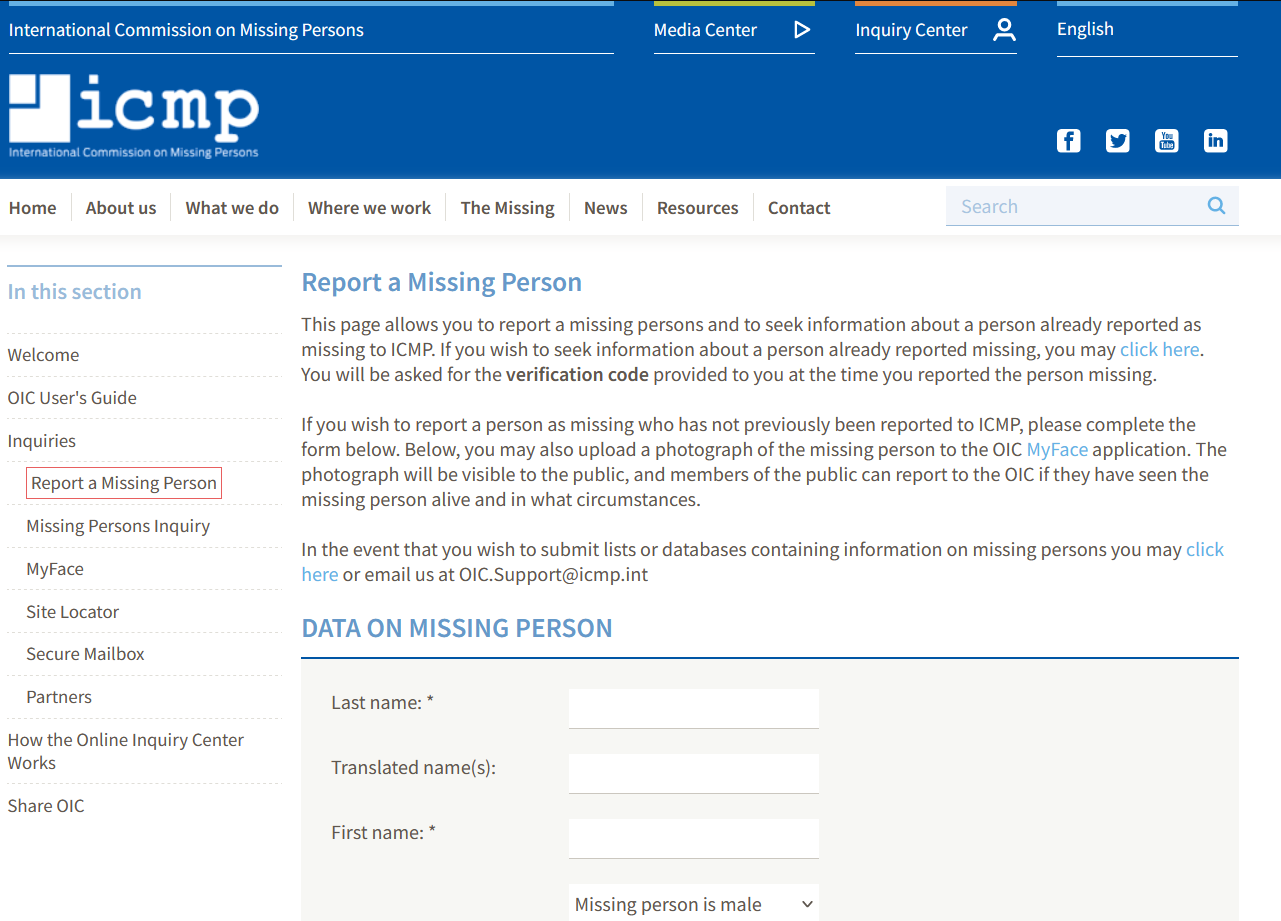
\includegraphics[scale=0.5]{slike/ICMP.png} %veličina slike u odnosu na originalnu datoteku i pozicija slike
			         \centering
			         \caption{Prijava nestale osobe preko ICMP}
			         \label{fig:promjene}
		      \end{figure}


            \begin{figure}[H]
			         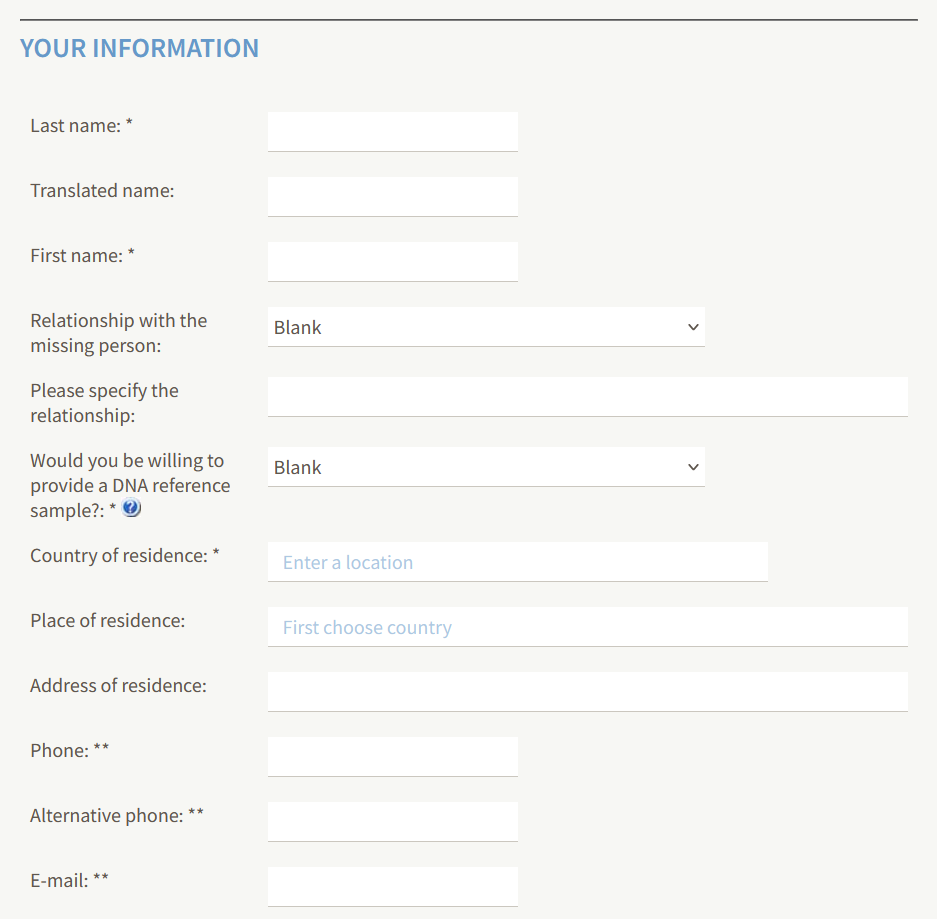
\includegraphics[scale=0.5]{slike/ICMP_2.png} %veličina slike u odnosu na originalnu datoteku i pozicija slike
			         \centering
			         \caption{Popunjavanje informacije korisnika}
			         \label{fig:promjene}
		      \end{figure}


            
			

            
			%\textit{mogućnost prilagodbe rješenja }
			%\textit{opseg projektnog zadatka}
			%\textit{moguće nadogradnje projektnog zadatka}
		
		%\textit{Za pomoć pogledati reference navedene u poglavlju „Popis literature“, a po potrebi konzultirati sadržaj na internetu koji nudi dobre smjernice u tom pogledu.}
		\eject
		
		\section{Primjeri u \LaTeX u}
		
		\textit{Ovo potpoglavlje izbrisati.}\\

		U nastavku se nalaze različiti primjeri kako koristiti osnovne funkcionalnosti \LaTeX a koje su potrebne za izradu dokumentacije. Za dodatnu pomoć obratiti se asistentu na projektu ili potražiti upute na sljedećim web sjedištima:
		\begin{itemize}
			\item Upute za izradu diplomskog rada u \LaTeX u - \url{https://www.fer.unizg.hr/_download/repository/LaTeX-upute.pdf}
			\item \LaTeX\ projekt - \url{https://www.latex-project.org/help/}
			\item StackExchange za Tex - \url{https://tex.stackexchange.com/}\\
		
		\end{itemize} 	


		
		\noindent \underbar{podcrtani tekst}, \textbf{podebljani tekst}, 	\textit{nagnuti tekst}\\
		\noindent \normalsize primjer \large primjer \Large primjer \LARGE {primjer} \huge {primjer} \Huge primjer \normalsize
				
		\begin{packed_item}
			
			\item  primjer
			\item  primjer
			\item  primjer
			\item[] \begin{packed_enum}
				\item primjer
				\item[] \begin{packed_enum}
					\item[1.a] primjer
					\item[b] primjer
				\end{packed_enum}
				\item primjer
			\end{packed_enum}
			
		\end{packed_item}
		
		\noindent primjer url-a: \url{https://www.fer.unizg.hr/predmet/proinz/projekt}
		
		\noindent posebni znakovi: \# \$ \% \& \{ \} \_ 
		$|$ $<$ $>$ 
		\^{} 
		\~{} 
		$\backslash$ 
		
		
		\begin{longtblr}[
			label=none,
			entry=none
			]{
				width = \textwidth,
				colspec={|X[8,l]|X[8, l]|X[16, l]|}, 
				rowhead = 1,
			} %definicija širine tablice, širine stupaca, poravnanje i broja redaka naslova tablice
			\hline \multicolumn{3}{|c|}{\textbf{naslov unutar tablice}}	 \\ \hline[3pt]
			\SetCell{LightGreen}IDKorisnik & INT	&  	Lorem ipsum dolor sit amet, consectetur adipiscing elit, sed do eiusmod  	\\ \hline
			korisnickoIme	& VARCHAR &   	\\ \hline 
			email & VARCHAR &   \\ \hline 
			ime & VARCHAR	&  		\\ \hline 
			\SetCell{LightBlue} primjer	& VARCHAR &   	\\ \hline 
		\end{longtblr}
		

		\begin{longtblr}[
				caption = {Naslov s referencom izvan tablice},
				entry = {Short Caption},
			]{
				width = \textwidth, 
				colspec = {|X[8,l]|X[8,l]|X[16,l]|}, 
				rowhead = 1,
			}
			\hline
			\SetCell{LightGreen}IDKorisnik & INT	&  	Lorem ipsum dolor sit amet, consectetur adipiscing elit, sed do eiusmod  	\\ \hline
			korisnickoIme	& VARCHAR &   	\\ \hline 
			email & VARCHAR &   \\ \hline 
			ime & VARCHAR	&  		\\ \hline 
			\SetCell{LightBlue} primjer	& VARCHAR &   	\\ \hline 
		\end{longtblr}
	


		
		
		%unos slike
		\begin{figure}[H]
			\includegraphics[scale=0.4]{slike/aktivnost.PNG} %veličina slike u odnosu na originalnu datoteku i pozicija slike
			\centering
			\caption{Primjer slike s potpisom}
			\label{fig:promjene}
		\end{figure}
		
		\begin{figure}[H]
			\includegraphics[width=\textwidth]{slike/aktivnost.PNG} %veličina u odnosu na širinu linije
			\caption{Primjer slike s potpisom 2}
			\label{fig:promjene2} %label mora biti drugaciji za svaku sliku
		\end{figure}
		
		Referenciranje slike \ref{fig:promjene2} u tekstu.
		
		\eject
		
	
	\chapter{Specifikacija programske potpore}
    \graphicspath{./dijagrami/}
		
	\section{Funkcionalni zahtjevi}
			
			\textbf{\textit{dio 1. revizije}}\\
			
			\textit{Navesti \textbf{dionike} koji imaju \textbf{interes u ovom sustavu} ili  \textbf{su nositelji odgovornosti}. To su prije svega korisnici, ali i administratori sustava, naručitelji, razvojni tim.}\\
				
			\textit{Navesti \textbf{aktore} koji izravno \textbf{koriste} ili \textbf{komuniciraju sa sustavom}. Oni mogu imati inicijatorsku ulogu, tj. započinju određene procese u sustavu ili samo sudioničku ulogu, tj. obavljaju određeni posao. Za svakog aktora navesti funkcionalne zahtjeve koji se na njega odnose.}\\
			
			
			\noindent \textbf{Dionici:}
			
			\begin{packed_enum}
				
				\item Neregistrirani korisnik
				\item Voditelj operacije				
				\item Kartograf
				\item Spasioc
				\item Administrator
				
			\end{packed_enum}
			
			\noindent \textbf{Aktori i njihovi funkcionalni zahtjevi:}
			
			
			\begin{packed_enum}
				\item  \underbar{Neregistrirani/neprijavljeni korisnik može:}
				
				\begin{packed_enum}
					
					\item poslati zahtjev za registraciju s potrebnim osobnim podacima: korisničko ime, fotografija, ime, prezime, lozinka, broj mobitela i adresa, i s ulogom za koju se prijavljuje
					\item prijaviti nestalu osobu s imenom, prezimenom, fotografijom i opisom
					\item komentirati prijavu o nestaloj osobi
					
					
				\end{packed_enum}
			
				\item  \underbar{Voditelj operacije može:}
				
				\begin{packed_enum}

                        \item imati sve ovlasti kao i neregistrirani korisnik
					\item zaključati prijavu o nestaloj osobi nakon što osoba bude pronađena
					\item obrisati prijavu o nestaloj osobi i komentare na prijavi
					\item definirati područja na karti koja je potrebno pretražiti i kartografirati
					\item imati pristup statistici humanitarne akcije
					\item mijenjati podatke u svom profilu

					
				\end{packed_enum}
				
				\item  \underbar{Kartograf može:}
				
				\begin{packed_enum}
    
					\item imati sve ovlasti kao i neregistrirani korisnik
					\item promijeniti status odabranog bloka na karti iz nezapočetog u aktivno, i iz aktivnog u provjeru
					\item promijeniti status odabranog bloka na karti iz provjera u aktivno ako posao nije dobro odrađen, te nastavljati uređivati područje
					\item dodavati nove građevine bloku sa statusom aktivno
					\item imati pristup statistici humanitarne akcije
					\item mijenjati podatke u svom profilu


					
				\end{packed_enum}
				
				\item  \underbar{Spasioc može:}
				
				\begin{packed_enum}

                        \item imati sve ovlasti kao i neregistrirani korisnik
					\item pregledavati kartu sa unesenim građevinama i promijeniti im status u pretraženo ili nepretraženo
					\item zaključati prijavu o nestaloj osobi nakon što osoba bude pronađena
					\item mijenjati podatke u svom profilu

				
				\end{packed_enum}
				
				\item  \underbar{Administrator može:}
				
				\begin{packed_enum}

                        \item imati sve ovlasti kao i neregistrirani korisnik
					\item potvrditi željena prava neregistriranog korisnika
					\item vidjeti popis registriranih korisnika i njihovih osobnih podataka
					\item mijenjati dodijeljena prava registriranih korisnika
					\item imati sva prava i ovlasti kao registrirani korisnici

				
				\end{packed_enum}
				
				
				
			\end{packed_enum}
			
			
			\eject 
			
			
				
			\subsection{Obrasci uporabe}
				
				\textbf{\textit{dio 1. revizije}}
				
				\subsubsection{Opis obrazaca uporabe}
					\textit{Funkcionalne zahtjeve razraditi u obliku obrazaca uporabe. Svaki obrazac je potrebno razraditi prema donjem predlošku. Ukoliko u nekom koraku može doći do odstupanja, potrebno je to odstupanje opisati i po mogućnosti ponuditi rješenje kojim bi se tijek obrasca vratio na osnovni tijek.}\\
					

					
					\noindent \underbar{\textbf{UC1 - Registracija u sustav}}
					\begin{packed_item}
	
						\item \textbf{Glavni sudionik: }Korisnik
						\item  \textbf{Cilj:} Registracija u sustavu
						\item  \textbf{Sudionici:} Baza podataka
						\item  \textbf{Preduvjet:} -
						\item  \textbf{Opis osnovnog tijeka:}
						
						\item[] \begin{packed_enum}
	
							\item Korisnik odabire opciju za registraciju u sustav
							\item Korisnik upisuje tražene osobne podatke i ulogu za koju se prijavljuje
							\item Korisnik prima obavijest o uspješno obavljenoj registraciji
						\end{packed_enum}
						
						\item  \textbf{Opis mogućih odstupanja:}
						
						\item[] \begin{packed_item}
	
							\item[2.a] Korisnik odabire već postojeće korisničko ime i/ili e-mail, ili unosi podatke u nedozvoljenom (neispravnom) formatu
							\item[] \begin{packed_enum}
								
								\item Sustav onemogućuje registraciju, te vraća korisnika na stranicu za registraciju
								\item Korisnik ispravlja pogrešno upisane podatke te registracija završava uspješno, ili odustaje od registracije
								
							\end{packed_enum}
							
							
						\end{packed_item}
					\end{packed_item}
					
					\noindent \underbar{\textbf{UC2 - Prijava u sustav}}
					\begin{packed_item}
	
						\item \textbf{Glavni sudionik: }Korisnik
						\item  \textbf{Cilj:}Stjecanje odgovarajućih ovlasti u aplikaciji
						\item  \textbf{Sudionici:} Baza podataka
						\item  \textbf{Preduvjet:} Uspješna registracija
						\item  \textbf{Opis osnovnog tijeka:}
						
						\item[] \begin{packed_enum}
	
							\item Korisnik unosi korisničko ime i lozinku
							\item Potvrda o ispravnosti unesenih podataka
							\item Dobivanje odgovarajućih ovlasti u aplikaciji
						\end{packed_enum}
						
						\item  \textbf{Opis mogućih odstupanja:}
						
						\item[] \begin{packed_item}
	
							\item[2.a] Neispravnost unesenog korisničkog imena i/ili lozinke
							\item[] \begin{packed_enum}
								
								\item Sustav obavještava korisnika o neuspjeloj prijavi u sustav i vraća ga na homepage
								
								
							\end{packed_enum}
							
						\end{packed_item}
					\end{packed_item}
					
				    \noindent \underbar{\textbf{UC3 - Pregled nestalih osoba}}
					\begin{packed_item}
	
						\item \textbf{Glavni sudionik: }Korisnik
						\item  \textbf{Cilj:} Pregled podataka nestalih osoba
						\item  \textbf{Sudionici:} Baza podataka
						\item  \textbf{Preduvjet:} Korisnik je prijavljen u sustav
						\item  \textbf{Opis osnovnog tijeka:}
						
						\item[] \begin{packed_enum}
	
							\item Korisnik odabire ekran "Nestali"
							\item Aplikacija daje prikaz podataka nestalih osoba
						\end{packed_enum}
						
					
					\end{packed_item}
					
				\noindent \underbar{\textbf{UC4 - Prijava nestale osobe}}
					\begin{packed_item}
	
						\item \textbf{Glavni sudionik: }Korisnik
						\item  \textbf{Cilj:} Prijaviti nestanak osobe
						\item  \textbf{Sudionici:} Baza podataka
						\item  \textbf{Preduvjet:} -
						\item  \textbf{Opis osnovnog tijeka:}
						
						\item[] \begin{packed_enum}
	
							\item Korisnik unosi podatke o nestaloj osobi u sustav
							
						\end{packed_enum}
						
						\item  \textbf{Opis mogućih odstupanja:}
						
						\item[] \begin{packed_item}
	
							\item[1.a] Prijava već prijavljene nestale osobe
							\item[] \begin{packed_enum}
								
								\item Sustav obavještava korisnika da je osoba već prijavljena kao nestala i vraća ga na stranicu "Nestali"
								
								
							\end{packed_enum}
							
							
						\end{packed_item}
					\end{packed_item}
					\noindent \underbar{\textbf{UC5 - Komentiranje prijave nestale osobe}}
					\begin{packed_item}
	
						\item \textbf{Glavni sudionik: }Korisnik
						\item  \textbf{Cilj:} Komentiranje prijave nestale osobe
						\item  \textbf{Sudionici:} Baza podataka
						\item  \textbf{Preduvjet:} -
						\item  \textbf{Opis osnovnog tijeka:}
						
						\item[] \begin{packed_enum}
	
							\item Korisnik piše komentar na prijavu o nestaloj osobi
							
						\end{packed_enum}
						
					
					\end{packed_item}
					\noindent \underbar{\textbf{UC6 - Zaključavanje prijave }}
					\begin{packed_item}
	
						\item \textbf{Glavni sudionik: }Spasioc ili voditelj operacije
						\item  \textbf{Cilj:} Zaključavanje prijave o nestaloj osobi
						\item  \textbf{Sudionici:} Baza podataka
						\item  \textbf{Preduvjet:} Osoba je pronađena
						\item  \textbf{Opis osnovnog tijeka:}
						
						\item[] \begin{packed_enum}
	
							\item Spasioc ili voditelj operacije odabire ekran "Nestali"
							\item Spasioc ili voditelj operacije zaključava prijavu o nestaloj osobi
							\item Status prijave mijenja se u "zaključana".
							\item Prijava se više ne prikazuje u sustavu
							
						\end{packed_enum}
						
					
					\end{packed_item}
					\noindent \underbar{\textbf{UC7 - Brisanje prijave}}
					\begin{packed_item}
	
						\item \textbf{Glavni sudionik: }Voditelj operacije
						\item  \textbf{Cilj:} Uklanjanje prijave o nestaloj osobi
						\item  \textbf{Sudionici:} Baza podataka
						\item  \textbf{Preduvjet:} Voditelj operacije je prijavljen u sustav
						\item  \textbf{Opis osnovnog tijeka:}
						
						\item[] \begin{packed_enum}
	
							\item Voditelj operacije odabire ekran "Nestali"
							\item Voditelj operacije odabire gumb "Obriši prijavu"
							\item Prijava o nestaloj osobi briše se iz baze podataka
							
						\end{packed_enum}
						
					
					\end{packed_item}
					\noindent \underbar{\textbf{UC8 - Brisanje komentara}}
					\begin{packed_item}
	
						\item \textbf{Glavni sudionik: }Voditelj operacije
						\item  \textbf{Cilj:} Brisanje komentara sa prijave o nestaloj osobi
						\item  \textbf{Sudionici:} Baza podataka
						\item  \textbf{Preduvjet:} Postoji barem 1 komentar na prijavi o nestaloj osobi
						\item  \textbf{Opis osnovnog tijeka:}
						
						\item[] \begin{packed_enum}
	
							\item Voditelj operacije odabire željenu prijavu o nestaloj osobi
							\item Voditelj operacije odabire gumb "Obriši komentar" za željeni komentar
							
						\end{packed_enum}
						
					
					\end{packed_item}
					\noindent \underbar{\textbf{UC9 - Prikaz karte}}
					\begin{packed_item}
	
						\item \textbf{Glavni sudionik: }Korisnik
						\item  \textbf{Cilj:} Prikaz područja na karti
						\item  \textbf{Sudionici:} Baza podataka
						\item  \textbf{Preduvjet:} Korisnik je prijavljen u sustav
						\item  \textbf{Opis osnovnog tijeka:}
						
						\item[] \begin{packed_enum}
	
							\item Nakon prijave korisniku je vidljiva karta sa označenim regijama i blokovima svih operacija

						\end{packed_enum}
					\end{packed_item}
					\noindent \underbar{\textbf{UC10 - Stvaranje operacije}}
					\begin{packed_item}
	
						\item \textbf{Glavni sudionik: }Voditelj operacije
						\item  \textbf{Cilj:} Definiranje područja koje je potrebno pretražiti
						\item  \textbf{Sudionici:} Baza podataka
						\item  \textbf{Preduvjet:} Voditelj operacije je prijavljen u sustav
						\item  \textbf{Opis osnovnog tijeka:}
						
						\item[] \begin{packed_enum}
	
							\item Voditelj operacije odabire ekran "Karta"  
							\item Voditelj operacije odabire gumb "Stvori novu operaciju"
							\item Voditelj operacije unosi potrebne podatke o operaciji: ime operacije i područje (regije i blokove) koje je potrebno pretražiti
							\item Podaci o stvorenoj operaciji spremaju se u bazu podataka
						\end{packed_enum}
						
						\item  \textbf{Opis mogućih odstupanja:}
						
						\item[] \begin{packed_item}
	
							\item[2.a] Stvorena je operacija s već postojećim imenom
							\item[] \begin{packed_enum}
								
								\item Sustav onemogućuje stvaranje nove operacije, te javlja grešku.

							\end{packed_enum}
							
						\end{packed_item}
					\end{packed_item}
					\noindent \underbar{\textbf{UC11 - Mijenjanje statusa bloka}}
					\begin{packed_item}
						
						\item \textbf{Glavni sudionik: }Kartograf
						\item  \textbf{Cilj:} Promjena statusa bloka
						\item  \textbf{Sudionici:} Baza podataka
						\item  \textbf{Preduvjet:} Kartograf je prijavljen u sustav
						\item  \textbf{Opis osnovnog tijeka:}
						
						\item[] \begin{packed_enum}
							
							\item Kartograf odabire ekran "Karta"
							\item Kartograf odabire blok na kojem želi raditi
							\item Kartograf odabire gumb "Promijeni status bloka"
							\item Kartograf mijenja status bloka iz "nezapočeto" u "aktivno" te potom uređuje blok 
							\item Kartograf mijenja status bloka iz "aktivno" u "provjera" nakon što je odradio posao
							\item Status bloka mijenja se iz "provjera" u "dovršeno" ako su dva kartografa provjerila odrađeni posao
							\item Promjena statusa bloka sprema se u bazu podataka
						\end{packed_enum}
						
						\item  \textbf{Opis mogućih odstupanja:}
						
						\item[] \begin{packed_item}
							
							\item[2.a] Kartograf odabire blok sa statusom "aktivan" kojeg uređuje drugi kartograf
							\item[] \begin{packed_enum}
								
								\item Nije mu dopušteno uređivanje bloka uz ispis prigodne poruke
								
							\end{packed_enum}
							
							\item[5.a] Kartograf smatra da posao nije dobro odrađen
							\item[] \begin{packed_enum}
								
								\item Kartograf mijenja status bloka iz "provjera" u "aktivno"
								
							\end{packed_enum}
							
						\end{packed_item}
					\end{packed_item}
					\noindent \underbar{\textbf{UC12 - Dodavanje građevine u blok}}
					\begin{packed_item}
						
						\item \textbf{Glavni sudionik: }Kartograf
						\item  \textbf{Cilj:} Dodavanje nove građevine u blok
						\item  \textbf{Sudionici:} Baza podataka
						\item  \textbf{Preduvjet:} Blok ima status "aktivan"
						\item  \textbf{Opis osnovnog tijeka:}
						
						\item[] \begin{packed_enum}
							
							\item Kartograf odabire ekran "Karta"
							\item Kartograf odabire blok na kojem želi unijeti građevinu
							\item Kartograf odabire gumb "Unesi novu građevinu"
							\item Kartograf unosi podatke o građevini
							\item Podaci o unesenoj građevini spremaju se u bazu podataka
						\end{packed_enum}
						
						\item  \textbf{Opis mogućih odstupanja:}
						
						\item[] \begin{packed_item}
							
							\item[4.a] Građevina s tim podacima već postoji
							\item[] \begin{packed_enum}
								
								\item Sustav onemogućava dodavanje građevine te javlja grešku
								
							\end{packed_enum}
							
						\end{packed_item}
					\end{packed_item}
					\noindent \underbar{\textbf{UC13 - Mijenjanje statusa građevini}}
					\begin{packed_item}
						
						\item \textbf{Glavni sudionik: }Spasioc
						\item  \textbf{Cilj:} Promjena statusa građevine
						\item  \textbf{Sudionici:} Baza podataka
						\item  \textbf{Preduvjet:} Spasioc je prijavljen u sustav
						\item  \textbf{Opis osnovnog tijeka:}
						
						\item[] \begin{packed_enum}
							
							\item Spasioc odabire ekran "Karta"
							\item Spasioc odabire građevinu kojoj želi promijeniti status
							\item Spasioc odabire gumb "Promijeni status građevine"
							\item Spasioc mijenja status u "pretraženo" ako je građevina pretražena ili u "nepretraženo" ako građevina nije pretražena
							\item Podaci o statusu građevine spremaju se u bazu podataka
							
						\end{packed_enum}
					
					\end{packed_item}
					\noindent \underbar{\textbf{UC14 - Zaključavanje operacije}}
					\begin{packed_item}
						
						\item \textbf{Glavni sudionik: }Voditelj operacije
						\item  \textbf{Cilj:} Zaključavanje područja koja su uspješno kartografirana i pretražena
						\item  \textbf{Sudionici:} Baza podataka
						\item  \textbf{Preduvjet:} Područje je uspješno pretraženo
						\item  \textbf{Opis osnovnog tijeka:}
						
						\item[] \begin{packed_enum}
							
							\item Voditelj operacije odabire ekran "Karta"
							\item Voditelj operacije klikne na operaciju koju želi zaključati
							\item Voditelj operacije odabire gumb "Zaključaj operaciju"
							\item Područje se više ne prikazuje kao područje koje je potrebno pretražiti
							
						\end{packed_enum}
					
					\end{packed_item}
					\noindent \underbar{\textbf{UC15 - Prikaz statistike}}
					\begin{packed_item}
						
						\item \textbf{Glavni sudionik: }Voditelj operacije ili kartograf
						\item  \textbf{Cilj:} Prikaz statistike humanitarne akcije
						\item  \textbf{Sudionici:} Baza podataka
						\item  \textbf{Preduvjet:} Voditelj operacije ili kartograf je prijavljen u sustav
						\item  \textbf{Opis osnovnog tijeka:}
						
						\item[] \begin{packed_enum}
							
							\item Voditelj operacije ili kartograf odabire ekran "Statistika"
							\item Prikazuje se broj završenih blokova, broj prijavljenih nestalih i broj pronađenih osoba, te broj pretraženih i nepretraženih građevina kroz vrijeme
							
						\end{packed_enum}
					
					\end{packed_item}
					\noindent \underbar{\textbf{UC16 - Prikaz registriranih korisnika}}
					\begin{packed_item}
						
						\item \textbf{Glavni sudionik: }Administrator
						\item  \textbf{Cilj:} Prikaz svih registriranih korisnika te njihovih osobnih podataka
						\item  \textbf{Sudionici:} Baza podataka
						\item  \textbf{Preduvjet:} Administrator je prijavljen u sustav
						\item  \textbf{Opis osnovnog tijeka:}
						
						\item[] \begin{packed_enum}
							
							\item Administrator odabire ekran "Admin page"
							\item Administratoru se prikazuje popis korisnika te njihovih osobnih podataka
							
						\end{packed_enum}
					
					\end{packed_item}
					\noindent \underbar{\textbf{UC17 - Mijenjanje prava korisnicima}}
					\begin{packed_item}
						
						\item \textbf{Glavni sudionik: }Administrator
						\item  \textbf{Cilj:} Mogućnost mijenjanja prava registriranim korisnicima
						\item  \textbf{Sudionici:} Baza podataka
						\item  \textbf{Preduvjet:} Administrator je prijavljen u sustav
						\item  \textbf{Opis osnovnog tijeka:}
						
						\item[] \begin{packed_enum}
							
							\item Administrator odabire ekran "Admin page"
							\item Administrator kod željenog korisnika odabire gumb "Promijeni prava"
							\item Administrator bira novo pravo tom korisniku
							\item Novi podaci o pravu korisnika spremaju se u bazu podataka
						\end{packed_enum}

					\end{packed_item}
					\noindent \underbar{\textbf{UC18 - Prikaz profila}}
					\begin{packed_item}
						
						\item \textbf{Glavni sudionik: }Korisnik
						\item  \textbf{Cilj:} Prikaz osobnih podataka korisnika
						\item  \textbf{Sudionici:} Baza podataka
						\item  \textbf{Preduvjet:} Korisnik je prijavljen u sustav
						\item  \textbf{Opis osnovnog tijeka:}
						
						\item[] \begin{packed_enum}
							
							\item Korisnik odabire ekran "Profile page"
							\item Korisniku se prikazuju njegovi osobni podaci
						\end{packed_enum}
					
					\end{packed_item}
					\noindent \underbar{\textbf{UC19 - Uređivanje profila}}
					\begin{packed_item}
						
						\item \textbf{Glavni sudionik: }Korisnik
						\item  \textbf{Cilj:} Mogućnost uređivanja osobnih podataka
						\item  \textbf{Sudionici:} Baza podataka
						\item  \textbf{Preduvjet:} Korisnik je prijavljen u sustav
						\item  \textbf{Opis osnovnog tijeka:}
						
						\item[] \begin{packed_enum}
							
							\item Korisnik odabire ekran "Profile page"
							\item Korisnik kod podatka koji želi promijeniti odabire gumb "Uredi"
							\item Korisnik unosi novi podatak na to mjesto
							\item Novi podaci o korisniku spremaju se u bazu podataka
						\end{packed_enum}
						
					\end{packed_item}
					\noindent \underbar{\textbf{UC20 - Potvrda registracije}}
					\begin{packed_item}
						
						\item \textbf{Glavni sudionik: }Administrator
						\item  \textbf{Cilj:} Mogućnost potvrde ili odbijanja registracije korisnika
						\item  \textbf{Sudionici:} Baza podataka
						\item  \textbf{Preduvjet:} Administrator je prijavljen u sustav
						\item  \textbf{Opis osnovnog tijeka:}
						
						\item[] \begin{packed_enum}
							
							\item Administrator odabire ekran "Admin page"
							\item Administrator odabire gumb "Zahtjevi za registraciju"
							\item Administrator odabire gumb "Potvrdi registraciju"
							\item Podaci o korisniku spremaju se u bazu podataka
						\end{packed_enum}
						
						\item  \textbf{Opis mogućih odstupanja:}
						
						\item[] \begin{packed_item}
							
							\item[3.a] Administrator ne želi potvrditi registraciju
							\item[] \begin{packed_enum}
								
								\item Administrator odabire gumb "Odbij registraciju"
								\item Zahtjev za registracijom je odbijen te se korisniku ispisuje prigodna poruka
								
							\end{packed_enum}
							
						\end{packed_item}
					\end{packed_item}
				
				\subsubsection{Dijagrami obrazaca uporabe}
					
					\textit{Prikazati odnos aktora i obrazaca uporabe odgovarajućim UML dijagramom. Nije nužno nacrtati sve na jednom dijagramu. Modelirati po razinama apstrakcije i skupovima srodnih funkcionalnosti.}
					
					
					\begin{figure}[H]      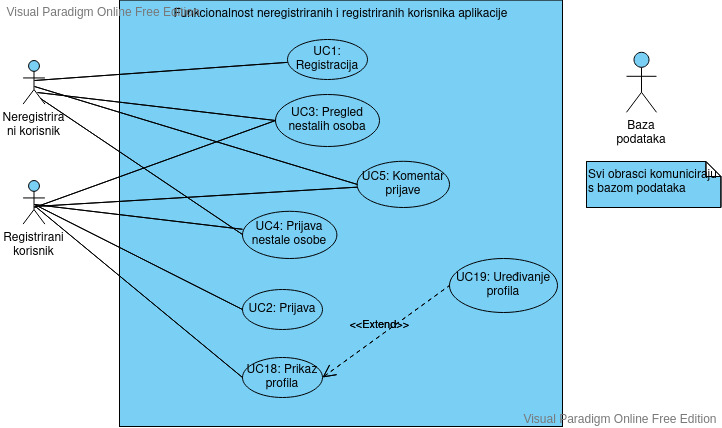
\includegraphics[width=\linewidth]{dijagrami/UML1.vpd.jpg}
					\caption{Dijagram obrasca uporabe, funkcionalnost neregistriranih i registriranih korisnika aplikacije}
	                \end{figure}
	                
				    \begin{figure}[h!] 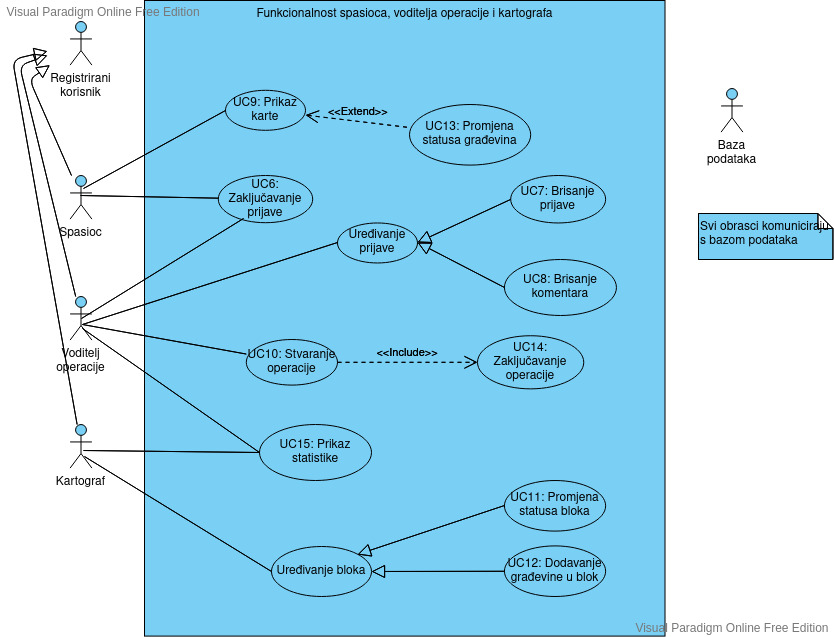
\includegraphics[width=\linewidth]{dijagrami/UML2.vpd.jpg}
				    \caption{Dijagram obrasca uporabe, funkcionalnost spasioca, voditelja operacije i kartografa}
				    \end{figure}
				    
				    \begin{figure}[h!] 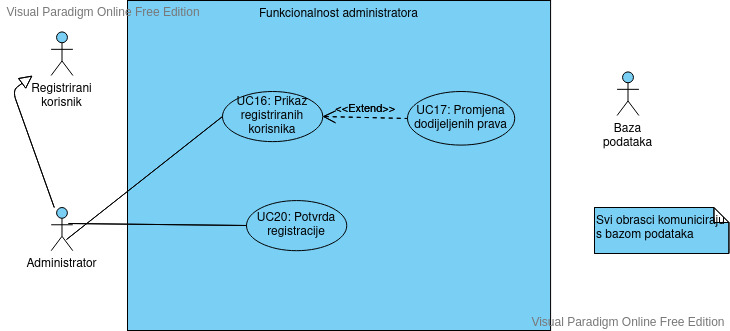
\includegraphics[width=\linewidth]{dijagrami/UML3.vpd.jpg} 
				    \caption{Dijagram obrasca uporabe, funkcionalnost administratora}
				    \end{figure} 
					
				\eject		
				
				\subsection{Sekvencijski dijagrami}
				
				\textbf{Obrazac uporabe UC4 - Prijava nestale osobe}
    
                Klijent šalje zahtjev za prijavu nestale osobe. Poslužitelj prikazuje obrazac za prijavu. Klijent ispunjava obrazac (ime, prezime, fotografija i opis) za prijavu nestale osobe. Poslužitelj dohvaća podatke iz baze te provjerava je li nova prijavljena osoba u bazi. Ako osoba dosad nije prijavljena, zapisuje se u bazu nestalih te sustav šalje potvrdu i prikaz prijave. Ukoliko je osoba već prijavljena, poslužitelj obavještava klijenta uz poruku.

                \begin{figure}[H] 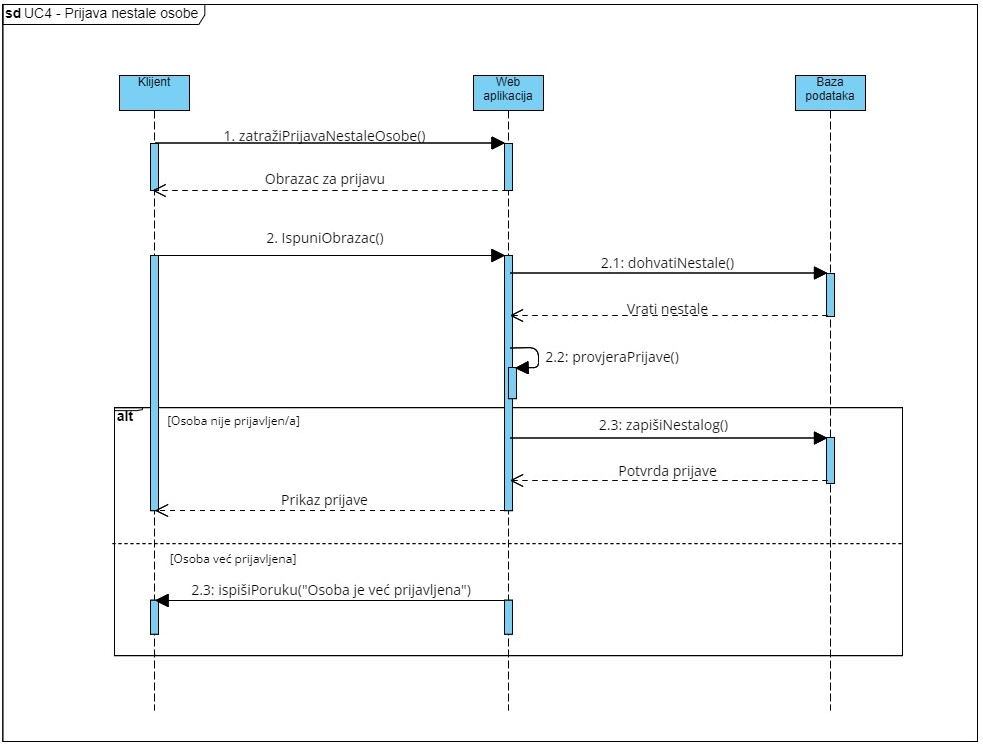
\includegraphics[width=\linewidth]{./dijagrami/PrijavaNestalog.jpg}
				    \caption{Sekvencijski dijagram za UC4 - Prijava nestale osobe}
				    \end{figure}

                \eject

                \textbf{Obrazac uporabe UC10 - Stvaranje operacije}

                Klijent šalje zahtjev za stvaranje operacije. Sustav provjerava je li korisnik voditelj. Ako korisnik nije voditelj, poslužitelj će ispisati poruku da nema ovlaštenje za stvaranje nove operacije, a ukoliko je, poslat će obrazac za stvaranje nove operacije. Klijent stvara novu operaciju, tj. upisuje ime operacije i područje (regije i blokove) koje je potrebno pretražiti. Poslužitelj dohvaća podatke iz baze te provjerava postoji li već operacija s tim imenom. Ako ne postoji, nova stvorena operacija se zapisuje u bazu podataka te sustav šalje potvrdu i prikaz nove operacije. Ukoliko  već postoji operacija s tim imenom, sustav javlja grešku da je stvorena operacija s već postojećim imenom.
                
                \begin{figure}[H] 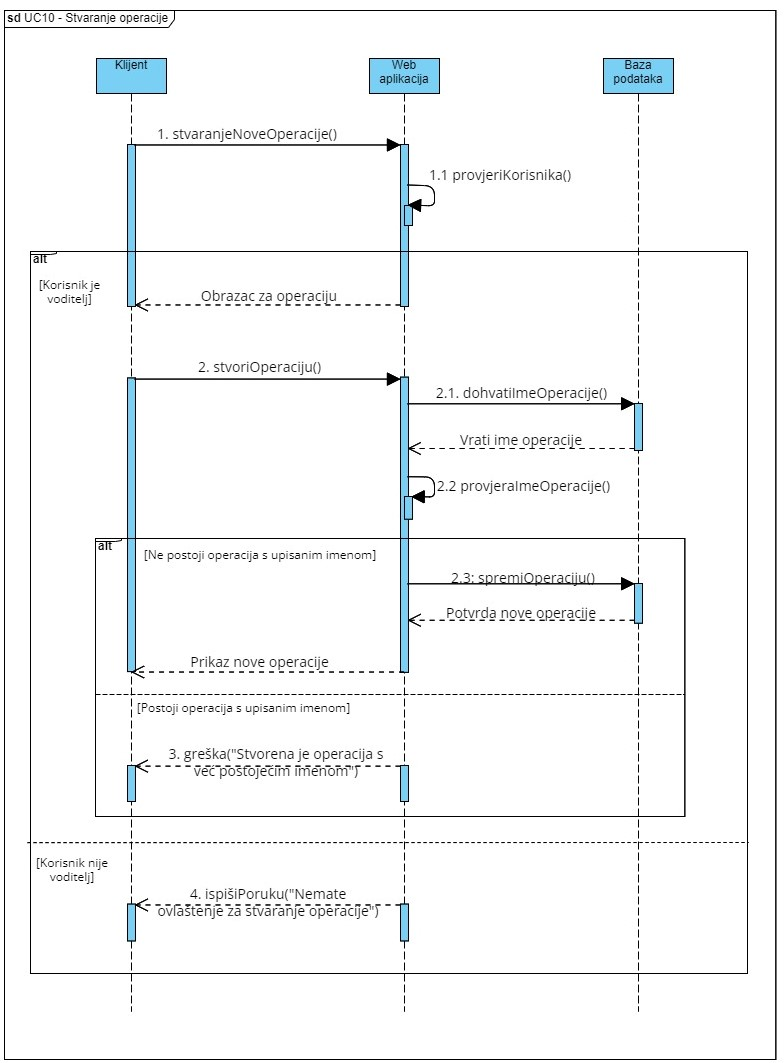
\includegraphics[width=\linewidth]{./dijagrami/StvaranjeOperacije.jpg}
				    \caption{Sekvencijski dijagram za UC10 - Stvaranje operacije}
				    \end{figure}

            	\eject

				\textbf{Obrazac uporabe UC11 - Mijenjanje statusa bloka}

                Klijent šalje zahtjev za prikaz karte. Web poslužitelj prikazuje kartu s opcijama, oviseći o korisniku. Klijent šalje zahtjev za prikaz bloka koji želi uređivati. Sustav dohvaća iz baze taj blok i prikazuje ga klijentu. Klijent šalje zahtjev za promjenu statusa bloka. Web poslužitelj provjerava status bloka te ako je blok aktivan ispisuje poruku da nije dopušteno uređivanje bloka. Ako je blok u statusu "Nezapočeto", klijent šalje zahtjev za promjenu statusa u "Aktivan". Sustav zapisuje status u bazu te prikazuje potvrdu promjene statusa. Ako je blok u statusu "Provjera", kartograf može smatrati da je posao dobro obavljen ili nije. Ukoliko kartograf smatra da posao nije dobro obavljen, šalje zahtjev sustavu za promjenu statusa bloka u "Aktivan" koji se zapisuje u bazu. Ukoliko kartograf smatra da je posao dobro obavljen, potvrđuje blok. Ukoliko su 2 kartografa potvrdila blok, mijenja se status bloka u "Završeno" i zapisuje u bazu. Kad je status bloka aktivan klijent može uređivati blok što se nastavlja u UC12 - Dodavanje građevine u blok. Kad je kartograf gotov s uređivanjem bloka, šalje zahtjev za promjenu statusa u "Provjera". Sustav zapisuje promjenu u bazu te šalje potvrdu.

                \begin{figure}[H] 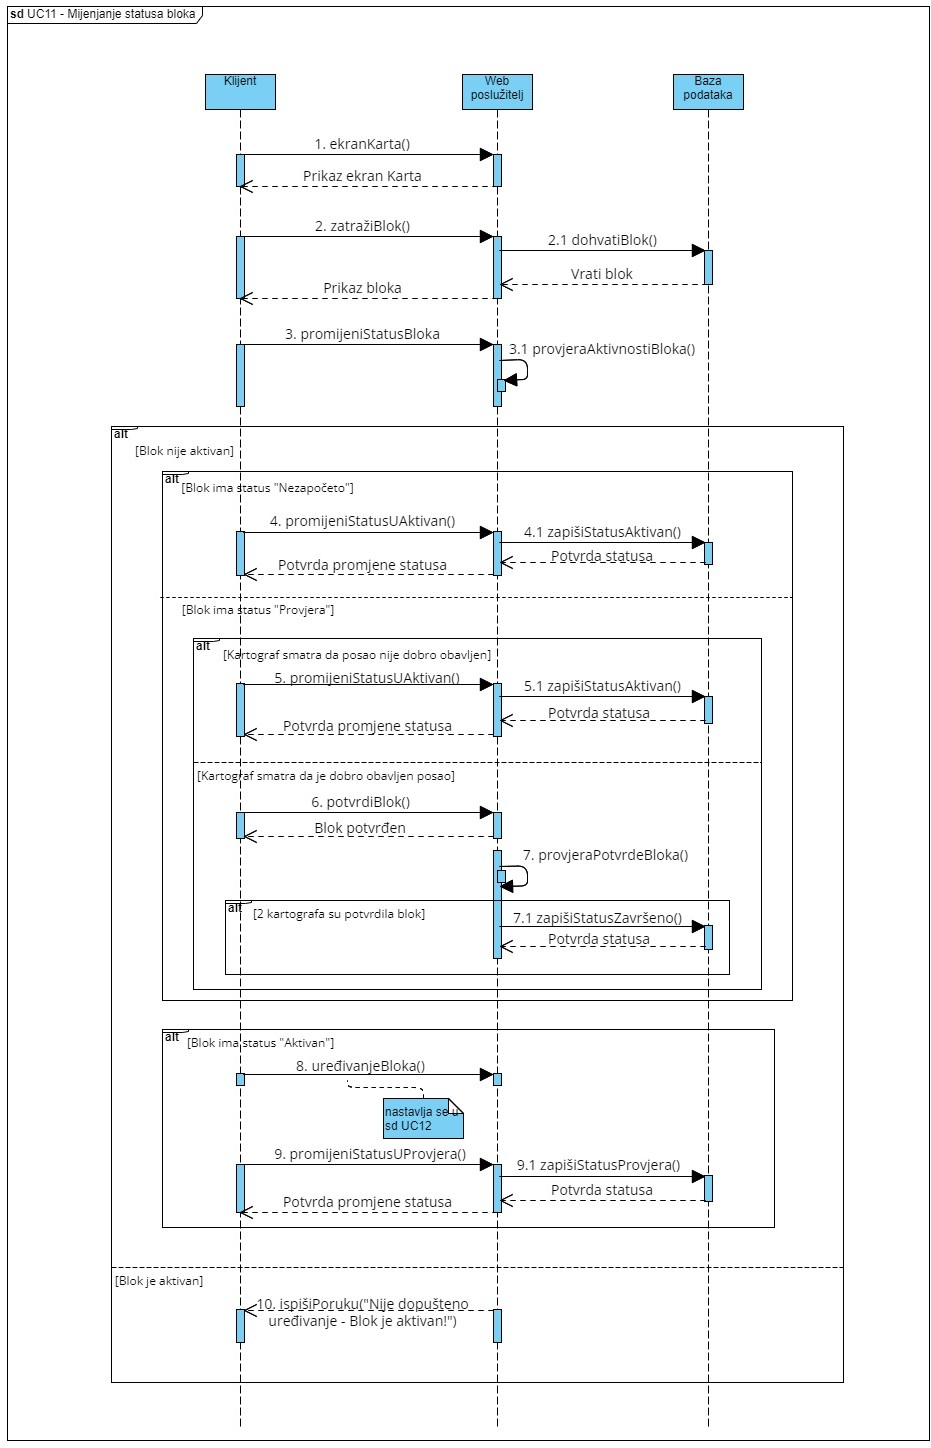
\includegraphics[width=\linewidth]{./dijagrami/MijenjanjeStatusaBloka.jpg}
				    \caption{Sekvencijski dijagram za UC11 - Mijenjanje statusa bloka}
				    \end{figure}
                
                \eject

                \textbf{Obrazac uporabe UC20 - Potvrda registracije}

                Klijent šalje zahtjev za otvaranjem ekrana admin. Sustav provjerava je li korisnik administrator te ako nije, web poslužitelj ispisuje poruku da nema ovlaštenja za pristup Admin pageu. Ukoliko je korisnik administrator, sustav prikazuje ekran Admin. Klijent šalje zahtjev za nepotvrđene registracije. Sustav dohvaća iz baze nepotvrđene korisnike te ih prikazuje. Ako administrator želi potvrditi registraciju, šalje zahtjev sustavu koji zapisuje zapisuje potvrdu korisnika u bazu. Sustav prikazuje potvrdu novog korisnika. Ukoliko administrator ne želi potvrditi registraciju, šalje zahtjev sustavu. Sustav briše korisnika iz baze te šalje potvrdu odbijene registracije. 

                \begin{figure}[H] 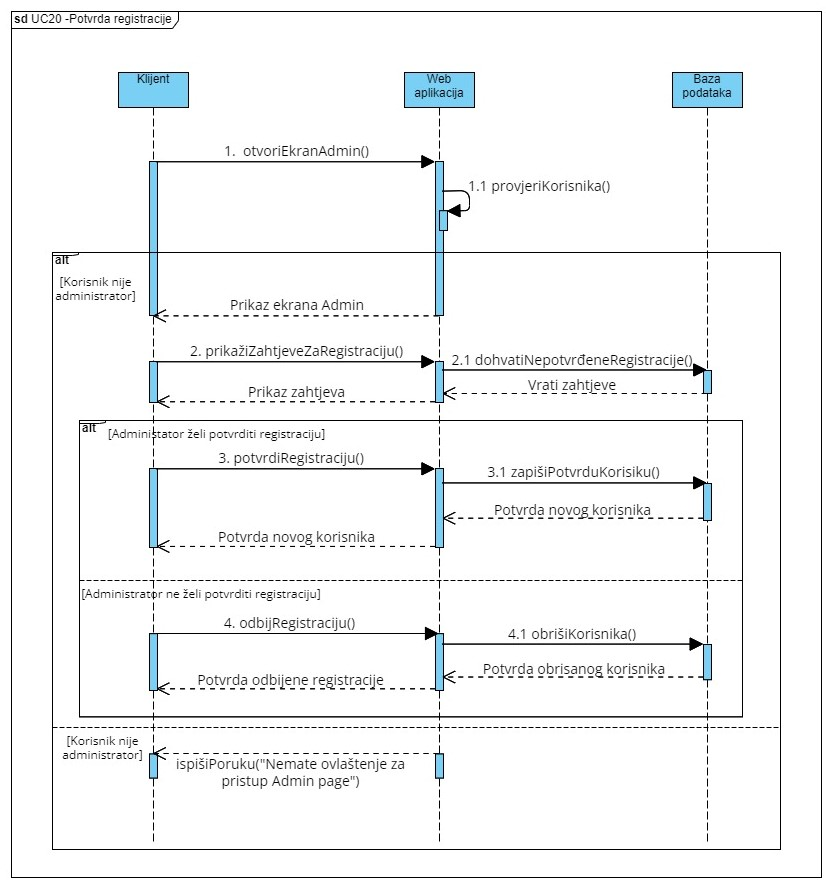
\includegraphics[width=\linewidth]{./dijagrami/PotvrdaRegistracije.jpg}
				    \caption{Sekvencijski dijagram za UC20 - Potvrda registracije}
				    \end{figure}
            \eject
	
		\section{Ostali zahtjevi}
		
			\textbf{\textit{dio 1. revizije}}\\
		 
			 \textit{Nefunkcionalni zahtjevi i zahtjevi domene primjene dopunjuju funkcionalne zahtjeve. Oni opisuju \textbf{kako se sustav treba ponašati} i koja \textbf{ograničenja} treba poštivati (performanse, korisničko iskustvo, pouzdanost, standardi kvalitete, sigurnost...). Primjeri takvih zahtjeva u Vašem projektu mogu biti: podržani jezici korisničkog sučelja, vrijeme odziva, najveći mogući podržani broj korisnika, podržane web/mobilne platforme, razina zaštite (protokoli komunikacije, kriptiranje...)... Svaki takav zahtjev potrebno je navesti u jednoj ili dvije rečenice.}
			 
			 \begin{itemize}
			 	\item Učitavanje početne stranice, stranice prijave korisnika ili nestalih osoba ne smije trajati duže od nekoliko sekundi
			 	\item Izgled aplikacije treba biti jednostavan kako bi se novi korisnici s lakoćom služili njezinim funkcionalnostima bez dodatnih pomagala (\textit{user-friendly})
			 	\item Proces prijave ili registracije korisnika ne smije trajati duže od nekoliko sekundi
			 	\item Sustav treba podržavati rad i operacije više korisnika u isto vrijeme bez ikakvih poteškoća
			 	\item Operacije vezane uz baze podataka trebaju biti brzo i efikasno izvršene
			 	\item Baza podataka treba biti pouzdana i dobro zaštićena
			 	\item U bazi podataka ne smiju postojati više operacija, korisnika te prijavljenih nestalih osoba s istim imenom
			 	\item Proces prijave nestale osobe ne smije predugo trajati
			 	\item Sustav treba podržavati korištenje dijakritičkih znakova pri unosu imena osoba ili operacija
			 	\item Promjena statusa ili faza blokova u bilo kojem smjeru ne smije narušavati funkcionalnost sustava
			 \end{itemize}
			 
			 
			 
	

	\chapter{Arhitektura i dizajn sustava}


               \textit{Arhitektura sustava može se podijeliti  na tri podsustava: }

              \begin{packed_item}
               \item  Web  preglednik
                \item   Web aplikacija
                \item    Baza Podataka

                \end{packed_item}

                 \begin{figure}[H]
                     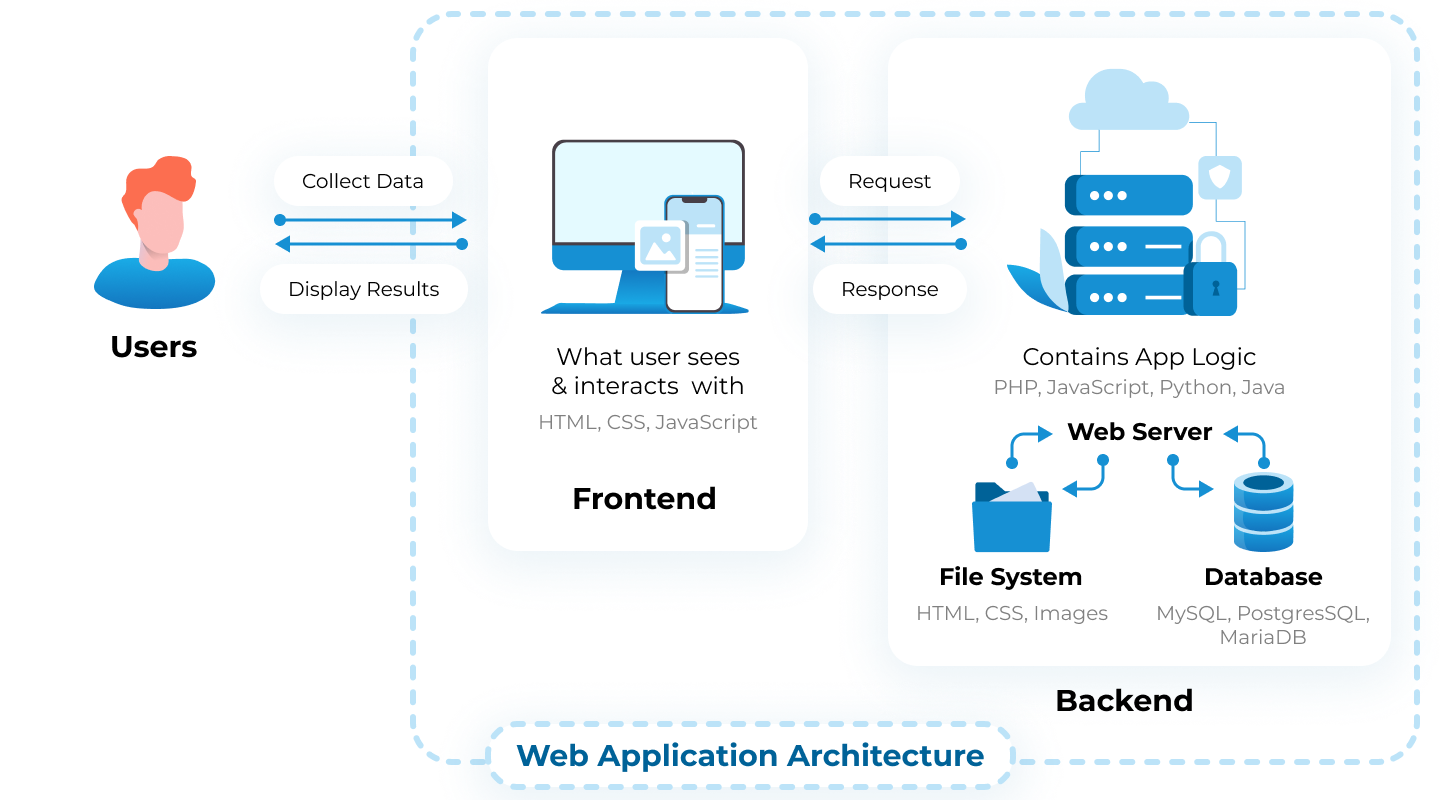
\includegraphics[width=7cm, height=5cm ]{./slike/arhitektura.png}
                      \centering
                      \caption{Arhitektura sustava}
                  \end{figure}


                  \textbf{Web preglednik} je aplikacija za prikaz web stranica. Kada korisnik posjeti neku web stranicu, internetski preglednik zatraži podatke
                                 sa web poslužitelja, koje interpretira i prikaže na zaslon računala ili nekog drugog pametnog uređaja.

                  \textbf{Web poslužitelj} osnovni podsustav u izradi web aplikacije. Njegova uloga u sustavu je komunikacija korisnika(web preglednika) s 
                                 aplikacijom. Komunikacija se ostvaruje preko HTTP (engl. Hyper Text Transfer Protocol) protokola. Uloga HTTP protokola je prijenos 
                                 sadržaja s poslužitelja na preglednik, koji dalje odrađuje svoj posao.
                            
                                Korisnik preko preglednika, koristi korisničko sučelje, te tako šalje HTTP zahtjeve na poslužitelj. Neki od zahtjeva su HTTP GET, HTTP POST 
                                itd. Svaki takav zahtjev u 99 \% slučajeva na poslužitelju izaziva, njegovu komunikaciju s \underbar{bazom podataka}.

                  \textbf{Baza podataka} je skup međusobno povezanih podataka, pohranjeni u vanjskoj memoriji računala. Njezina uloga u sustavu je brza i efikasna
                                 pohrana podataka, koji se propagiraju iz sloja web preglednika, preko web poslužitelja.

                  \textit{Web aplikacija se najčešće dijeli na dva dijela: }

                               \begin{packed_item}
              			 \item  \textbf{Front-end} koji je zadužen za razvoj korsicničkog iskustva na webu.
                		\item    \textbf{Back-end} koji je zadužen za obradu i spremanje podataka, koji dođu sa frontenda.

              		       \end{packed_item}

                                Tehnologije koje smo uzeli za razvoj web aplikacije su React.js za Front-end u razvojnom okruženju Microsoft Visual Studio Code, te .NET za Back-end u razvojnom okruženju Microsoft Visual Studio.
                                Uz .Net na back-endu, smo uzeli SQL server za bazu podataka. 
                                Arhitektura sustava će biti bazirana na MVC(engl. Model-View-Controller) konceptu.

                      \textbf{MVC} model sastoji se od tri komponenti: 
                                  
                               \begin{packed_item}
             			  \item \textbf{Model} -  komponenta modela koja je zadužena za dohvat i manipulacijom podataka. Često za obavljanje svojih zadaća koristi bazu podataka.
                		  \item  \textbf{View} -   komponenta kojoj je zadaća prikaz dobivenih podataka korisniku.
               		           \item  \textbf{Controller} - komponenta zadužena za primanje zahtjeva od korisnika, koje dalje propagira komponenti Model.

                                \end{packed_item}
                  
                    \begin{figure}[H]
                     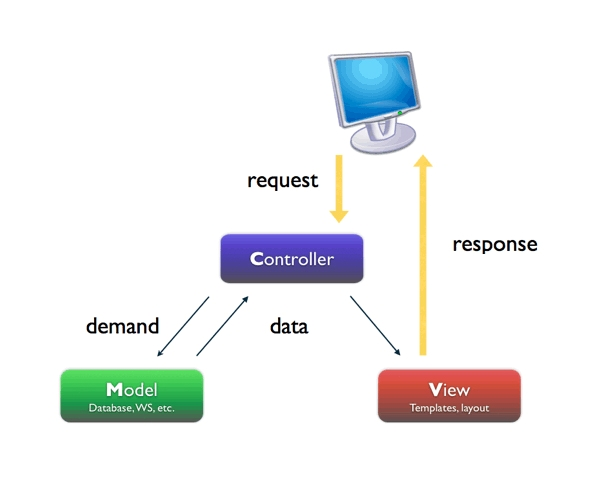
\includegraphics[width=7cm, height=5cm ]{./slike/mvc.jpg}
                      \centering
                      \caption{MVC model}
                    \end{figure}
                    
                                 

			
		\section{Baza podataka}

             Za potrebe našeg sustava koristimo relacijsku Microsoft SQL Server bazu podataka koja svojom strukturom olakšava modeliranje stvarnog svijeta. Gradivna jedinka baze je relacija, odnosno tablica koja je definirana svojim imenom i skupom atributa. Zadaća baze podataka je brza i jednostavna pohrana te izmjena i dohvat podataka za daljnju obradu.
        Baza podataka ove aplikacije sastoji se od sljedećih entiteta: \\
        \\
        \-\hspace{1cm} • Users \\
        \-\hspace{1cm} • Role \\
        \-\hspace{1cm} • Missing Report \\
        \-\hspace{1cm} • Comment \\
        \-\hspace{1cm} • Operation \\
        \-\hspace{1cm} • Area \\
        \-\hspace{1cm} • Region \\
        \-\hspace{1cm} • Block \\
        \-\hspace{1cm} • Building \\
        \-\hspace{1cm} • Point \\
			

			\subsection{Opis tablica}

\textbf{Users} Ovaj entitet sadrži sve važne informacije o korisniku aplikacije. Sadrži atribute: korisničko ime, OIB, ime, prezime, fotografiju, broj telefona, adresu elektroničke pošte, lozinku, ID uloge korisnika te status je li potvrđen. Ovaj entitet u vezi je \textit{Many-to-One} s entitetom Role preko atributa identifikatora uloge, u vezi \textit{One-To-Many} s entitetom Operation preko atributa identifikatora osobe, u vezi \textit{One-to-Many} s entitetom Comment preko atributa identifikatora osobe, u vezi \textit{One-To-Many} s entitetom Area preko atributa identifikatora osobe te u vezi \textit{One-To-Many} s entitetom Block preko atributa identifikatora osobe. 
				\begin{longtblr}[
					label=none,
					entry=none
					]{
						width = \textwidth,
						colspec={|X[6,l]|X[6, l]|X[20, l]|}, 
						rowhead = 1,
					} %definicija širine tablice, širine stupaca, poravnanje i broja redaka naslova tablice
					\hline \multicolumn{3}{|c|}{\textbf{Users}}	 \\ \hline[3pt]
					Username & VARCHAR	&  	korisničko ime korisnika  	\\ \hline
					\SetCell{LightGreen}OIB	& BIGINT & jedinstveni identifikator osobe   	\\ \hline 
					FirstName & VARCHAR & ime korisnika  \\ \hline 
					LastName & VARCHAR	& prezime korisnika 		\\ \hline
					Photo & VARCHAR & fotografija korisnika \\ \hline 
				    PhoneNumber & VARCHAR & telefonski broj korisnika  	\\ \hline 
					EMail & VARCHAR & adresa elektroničke pošte korisnika  	\\ \hline
					Password & VARCHAR & hash lozinke  	\\ \hline
                    \SetCell{LightBlue}RoleId & INT & identifikator uloge  	\\ \hline
                    Confirmed & BIT & status je li administrator potvrdio korisnika  	\\ \hline
				\end{longtblr}
				
\textbf{Role} Ovaj entitet sadrži sve važne informacije o ulogama korisnika aplikacije. Sadrži atribute ID uloge i ime uloge. Ovaj entitet u vezi je \textit{One-to-Many} s entitetom Users preko atributa identifikatora uloge. 
				\begin{longtblr}[
					label=none,
					entry=none
					]{
						width = \textwidth,
						colspec={|X[6,l]|X[6, l]|X[20, l]|}, 
						rowhead = 1,
					} %definicija širine tablice, širine stupaca, poravnanje i broja redaka naslova tablice
					\hline \multicolumn{3}{|c|}{\textbf{Role}}	 \\ \hline[3pt]
					\SetCell{LightGreen}Id & INT	&  jedinstveni identifikator uloge  	\\ \hline
					Name	& VARCHAR &  naziv uloge 	\\ \hline
				\end{longtblr}
			
\textbf{Missing Report} Ovaj entitet sadrži sve važne informacije o prijavama nestalih osoba. Sadrži atribute: ID prijave, ime osobe, prezime osobe, OIB osobe, fotografiju osobe, opis prijave, datum i vrijeme prijave te datum i vrijeme pronalaska. Ovaj entitet u vezi je \textit{One-to-Many} s entitetom Comment preko atributa identifikatora prijave nestale osobe.  
				\begin{longtblr}[
					label=none,
					entry=none
					]{
						width = \textwidth,
						colspec={|X[6,l]|X[6, l]|X[20, l]|}, 
						rowhead = 1,
					} %definicija širine tablice, širine stupaca, poravnanje i broja redaka naslova tablice
					\hline \multicolumn{3}{|c|}{\textbf{Missing Report}}	 \\ \hline[3pt]
					\SetCell{LightGreen}Id & INT	&  jedinstveni identifikator prijave nestale osobe  	\\ \hline
					FirstName	& VARCHAR &  ime nestale osobe 	\\ \hline
                    LastName	& VARCHAR &  prezime nestale osobe 	\\ \hline
                    OIB	& BIGINT &  jedinstveni identifikator nestale osobe 	\\ \hline
                    Photo	& VARCHAR &  fotografija nestale osobe 	\\ \hline
                    Description	& VARCHAR &  opis prijave nestale osobe 	\\ \hline
                    ReportedAt & DATETIME & datum i vrijeme prijave nestanka osobe   \\ \hline
                    FoundAt & DATETIME & datum i vrijeme pronalaska nestale osobe \\ \hline
				\end{longtblr}
			
\textbf{Comment} Ovaj entitet sadrži sve važne informacije o komentarima prijava nestalih osoba. Sadrži atribute ID komentara, ID prijave koja se komentira, sadržaj komentara, OIB korisnika. Ovaj entitet u vezi je \textit{Many-to-One} s entitetom Missing Report preko atributa identifikatora prijave nestale osobe i u vezi \textit{Many-to-One} s entitetom Users preko atributa identifikatora osobe. 
				\begin{longtblr}[
					label=none,
					entry=none
					]{
						width = \textwidth,
						colspec={|X[6,l]|X[6, l]|X[20, l]|}, 
						rowhead = 1,
					} %definicija širine tablice, širine stupaca, poravnanje i broja redaka naslova tablice
					\hline \multicolumn{3}{|c|}{\textbf{Comment}}	 \\ \hline[3pt]
					\SetCell{LightGreen}Id & INT	&  jedinstveni identifikator komentara  	\\ \hline
					\SetCell{LightBlue}ReportId	& INT &  jedinstveni identifikator prijave nestale osobe 	\\ \hline
                    Text & VARCHAR &  sadržaj komentara 	\\ \hline
                    \SetCell{LightBlue} UserOIB	& BIGINT &  jedinstveni identifikator osobe koja komentira 	\\ \hline
				\end{longtblr}

\textbf{Operation} Ovaj entitet sadrži sve važne informacije o operacijama. Sadrži atribute: ID operacije, status operacije i OIB voditelja operacije. Ovaj entitet u vezi je \textit{Many-to-One} s entitetom Users preko atributa identifikatora osobe te u vezi \textit{One-To-Many} s entitetom Region preko atributa identifikatora operacije. 
				\begin{longtblr}[
					label=none,
					entry=none
					]{
						width = \textwidth,
						colspec={|X[6,l]|X[6, l]|X[20, l]|}, 
						rowhead = 1,
					} %definicija širine tablice, širine stupaca, poravnanje i broja redaka naslova tablice
					\hline \multicolumn{3}{|c|}{\textbf{Operation}}	 \\ \hline[3pt]
					\SetCell{LightGreen}Id & INT	&  jedinstveni identifikator operacije\\ \hline
					Status	& VARCHAR &  status operacije 	\\ \hline
                    \SetCell{LightBlue}LeaderOIB	& BIGINT & jedinstveni identifikator voditelja operacije 	\\ \hline
				\end{longtblr}


\textbf{Area} Ovaj entitet sadrži sve važne informacije o područjima. Sadrži atribute: identifikator područja, datum i vrijeme nastanka područja, datum i vrijeme zatvaranja područja te identifikator osobe koja je zadnja uređivala područje. Ovaj entitet u vezi je \textit{Many-to-One} s entitetom Users preko atributa identifikatora osobe, u vezi \textit{One-To-Many} s entitetom Block preko atributa identifikatora područja, u vezi \textit{One-To-Many} s entitetom Building preko atributa identifikatora područja, u vezi \textit{One-To-Many} s entitetom Point preko atributa identifikatora područja te u vezi \textit{One-To-Many} s entitetom Region preko atributa identifikatora područja. 
				\begin{longtblr}[
					label=none,
					entry=none
					]{
						width = \textwidth,
						colspec={|X[9,l]|X[6, l]|X[20, l]|}, 
						rowhead = 1,
					} %definicija širine tablice, širine stupaca, poravnanje i broja redaka naslova tablice
					\hline \multicolumn{3}{|c|}{\textbf{Area}}	 \\ \hline[3pt]
					\SetCell{LightGreen}Id & INT	&  jedinstveni identifikator područja \\ \hline
					CreatedAt & DATETIME & datum i vrijeme nastanka područja \\ \hline
					ClosedAt & DATETIME & datum i vrijeme zatvaranja područja \\ \hline
					\SetCell{LightBlue}UpdatedLastByOIB	& BIGINT &  identifikator osobe koja je zadnja uređivala područje 	\\ \hline
				\end{longtblr}  
                
\textbf{Region} Ovaj entitet sadrži sve važne informacije o regiji. Sadrži atribute: identifikator regije te identifikator operacije. Ovaj entitet u vezi je \textit{Many-to-One} s entitetom Area preko atributa identifikatora regije, u vezi \textit{Many-To-One} s entitetom Operation preko atributa identifikatora operacije te u vezi \textit{One-To-Many} s entitetom Block preko atributa identifikatora regije. 
				\begin{longtblr}[
					label=none,
					entry=none
					]{
						width = \textwidth,
						colspec={|X[6,l]|X[6, l]|X[20, l]|}, 
						rowhead = 1,
					} %definicija širine tablice, širine stupaca, poravnanje i broja redaka naslova tablice
					\hline \multicolumn{3}{|c|}{\textbf{Region}}	 \\ \hline[3pt]
					\SetCell{LightGreen}AreaId & INT	&  jedinstveni identifikator regije \\ \hline
					\SetCell{LightBlue}OperationId	& INT &  jedinstveni identifikator operacije 	\\ \hline
				\end{longtblr}            
				
\textbf{Block} Ovaj entitet sadrži sve važne informacije o blokovima. Sadrži atribute: identifikator bloka, status bloka, identifikator regije te identifikator osobe koja uređuje blok. Ovaj entitet u vezi je \textit{Many-to-One} s entitetom Users preko atributa identifikatora osobe, u vezi \textit{Many-To-One} s entitetom Area preko atributa identifikatora bloka, u vezi \textit{Many-To-One} s entitetom Region preko atributa identifikatora regije te u vezi \textit{One-To-Many} s entitetom Building preko atributa identifikatora bloka. 
	          \begin{longtblr}[
	          	label=none,
	          	entry=none
	          	]{
	          		width = \textwidth,
	          		colspec={|X[6,l]|X[6, l]|X[20, l]|}, 
	          		rowhead = 1,
	          	} %definicija širine tablice, širine stupaca, poravnanje i broja redaka naslova tablice
	          	\hline \multicolumn{3}{|c|}{\textbf{Block}}	 \\ \hline[3pt]
	          	\SetCell{LightGreen}AreaId & INT	&  jedinstveni identifikator bloka \\ \hline
	          	Status & VARCHAR & status bloka \\ \hline
	          	\SetCell{LightBlue}RegionId & INT & jedinstveni identifikator regije \\ \hline
	          	\SetCell{LightBlue}ActiveForOIB	& BIGINT &  identifikator kartografa koji trenutno uređuje blok 	\\ \hline
	          \end{longtblr}  
				
\textbf{Building} Ovaj entitet sadrži sve važne informacije o građevinama. Sadrži atribute: identifikator građevine, identifikator bloka te status građevine. Ovaj entitet u vezi je \textit{Many-to-One} s entitetom Area preko atributa identifikatora građevine te u vezi \textit{Many-To-One} s entitetom Block preko atributa identifikatora bloka.
			\begin{longtblr}[
				label=none,
				entry=none
				]{
					width = \textwidth,
					colspec={|X[6,l]|X[6, l]|X[20, l]|}, 
					rowhead = 1,
				} %definicija širine tablice, širine stupaca, poravnanje i broja redaka naslova tablice
				\hline \multicolumn{3}{|c|}{\textbf{Building}}	 \\ \hline[3pt]
				\SetCell{LightGreen}AreaId & INT	&  jedinstveni identifikator građevine \\ \hline
				\SetCell{LightBlue}BlockId & INT & jedinstveni identifikator bloka \\ \hline
	          	Status & VARCHAR & status građevine \\ \hline
			\end{longtblr}

\textbf{Point} Ovaj entitet sadrži sve važne informacije o točkama i njihovim koordinatama. Sadrži atribute: identifikator točke, geografska širina, geografska dužina, identifikator područja te redni broj. Ovaj entitet u vezi je \textit{Many-to-One} s entitetom Area preko atributa identifikatora područja.
			\begin{longtblr}[
				label=none,
				entry=none
				]{
					width = \textwidth,
					colspec={|X[6,l]|X[6, l]|X[20, l]|}, 
					rowhead = 1,
				} %definicija širine tablice, širine stupaca, poravnanje i broja redaka naslova tablice
				\hline \multicolumn{3}{|c|}{\textbf{Point}}	 \\ \hline[3pt]
				\SetCell{LightGreen}Id & INT	&  jedinstveni identifikator točke \\ \hline
				Latitude & FLOAT & geografska širina točke \\ \hline
				Longitude & FLOAT & geografska dužina točke \\ \hline
				\SetCell{LightBlue}AreaId & INT & jedinstveni identifikator područja \\ \hline
				OrderNumber & INT & redni broj točke \\ \hline
			\end{longtblr}
			
			\subsection{Dijagram baze podataka}
				\begin{figure}[H]
					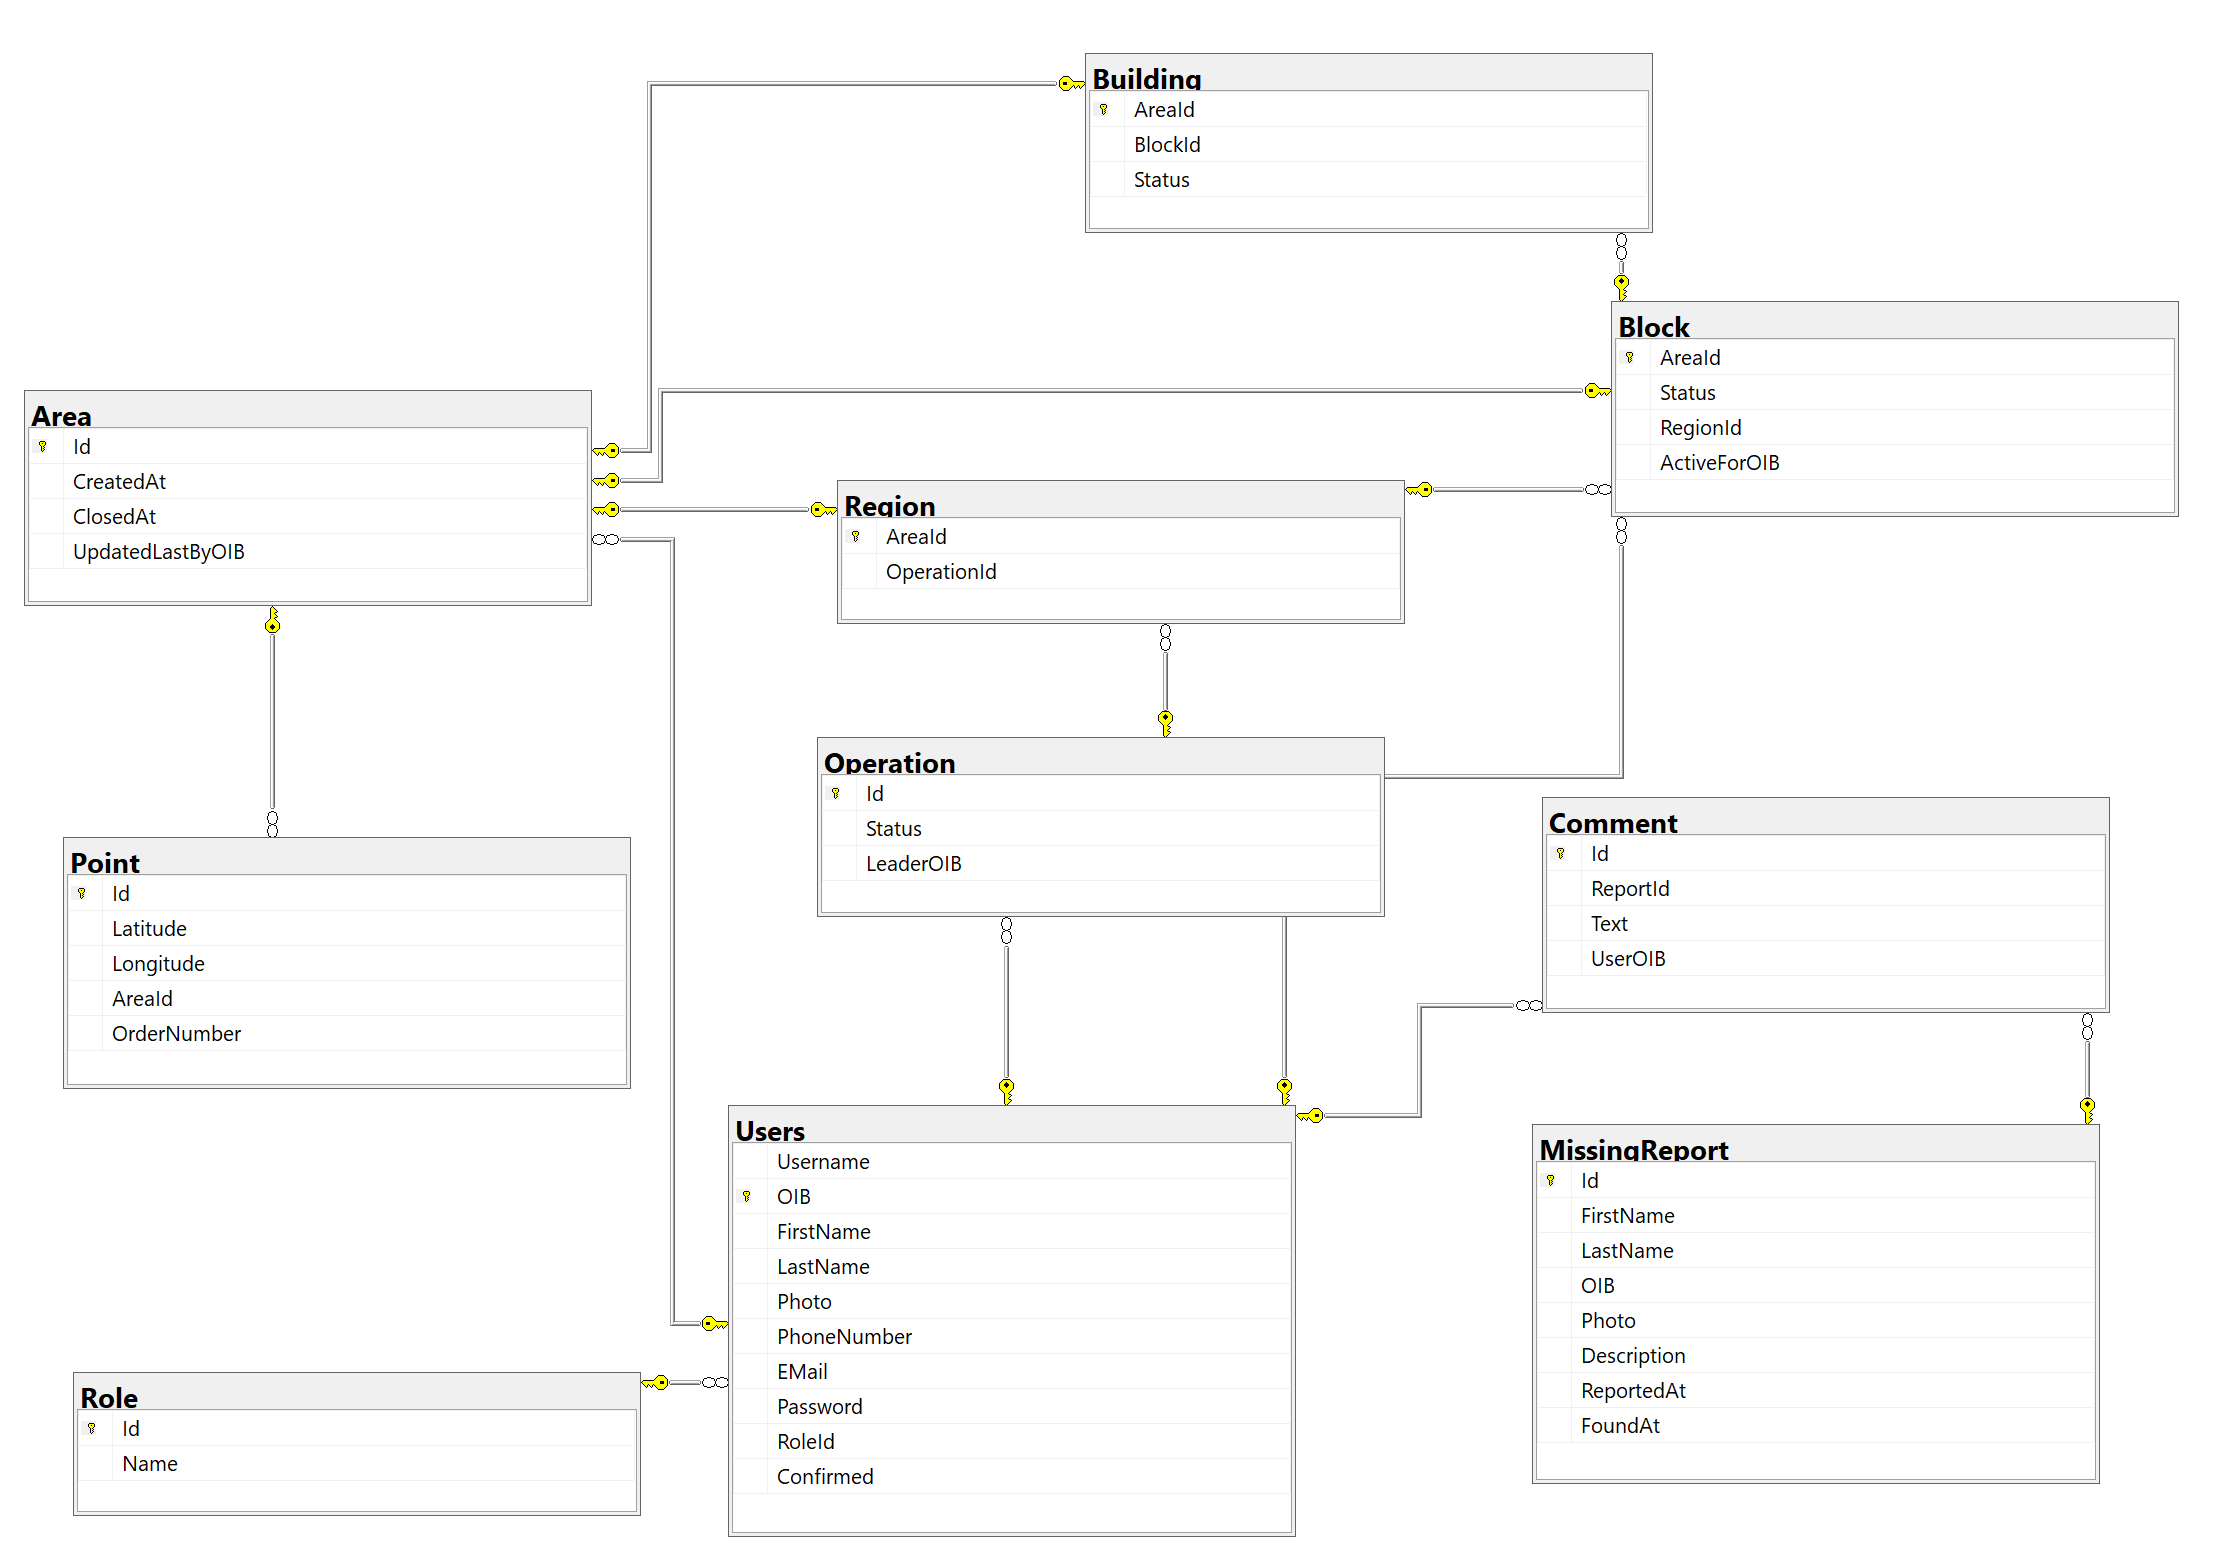
\includegraphics[width=15cm]{./slike/ERDijagram.png}
					 \centering
					 \caption{ER dijagram baze podataka}
				\end{figure}
			\eject
			
			
		\section{Dijagram razreda}
		
		Na slikama 4.4, 4.5, 4.6, 4.7 i 4.8 prikazani su razredi koji pripadaju \textit{backend} dijelu MVC arhitekure. Da bi se izbjegla prenapučenost, razredi su podijeljeni s obzirom na funkcionalnosti. Tako na prvom dijagramu imamo razrede vezane za registraciju i prijavu, na drugom su razredi vezani za prijave i komentare, na trećem se dijagramu nalaze svi razredi potrebni za karte i mapiranje, na četvrtom razredi vezani za korisnike i njihove uloge, a na petom su dijagramu smješteni razredi vezani za statistiku.
		
		Na slici 4.4 nalazi se dijagram koji prikazuje odnos Controllera, Modela i DTO-ova vezanih uz Login i Register. Vidimo da se, nakon registracije korisnika, podaci spremaju u bazu podataka, a također se iz RegisterControllera podaci šalju u UserDto. RegisterController i LoginController pomoću registerServicea i loginServicera realiziraju sučelja IRegister i ILogin te nasljeđuju njihove metode.
								
			\begin{figure}[h!] 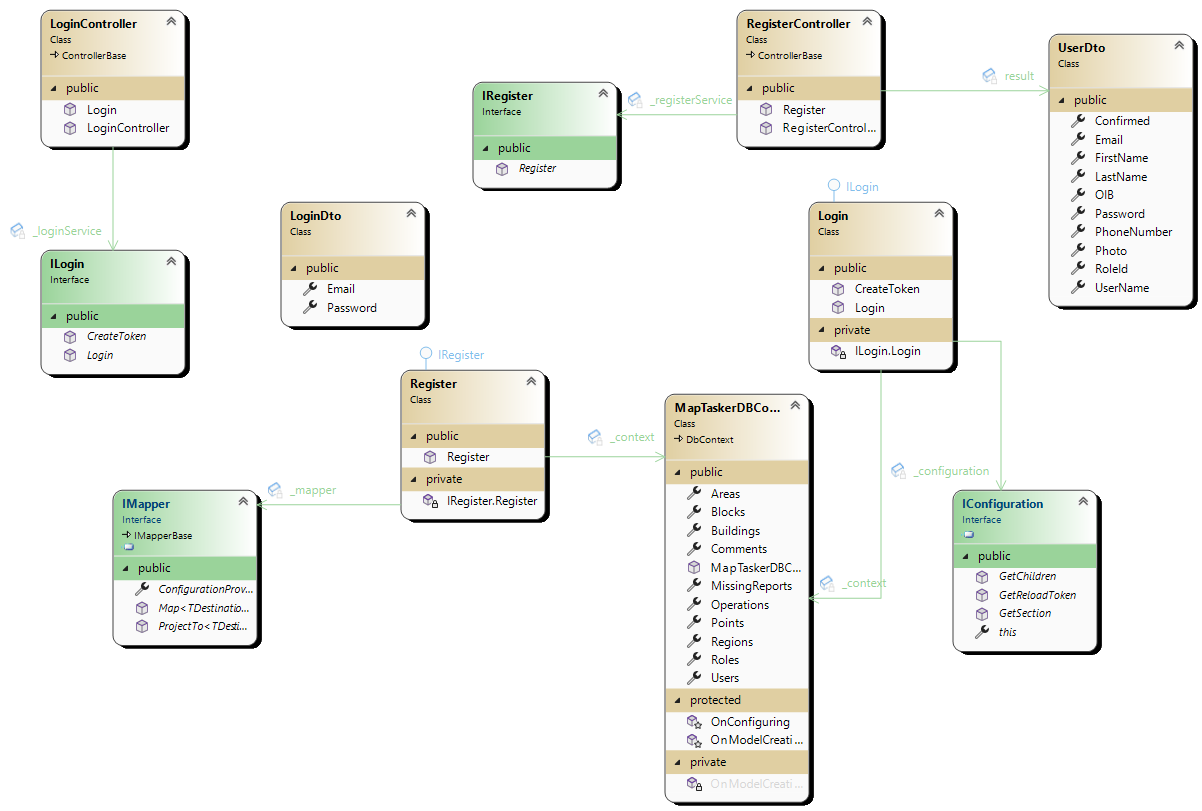
\includegraphics[width=\linewidth]{dijagrami/CD-LoginRegister.png}
				\caption{Dijagram razreda 1 - Register i Login}
			\end{figure}
		
		\eject
		
		Ovaj dijagram prikazuje prijave nestalih i komentare. Promatrajući Controllere, koji nasljeđuju sučelja, vidimo koje sve metode postoje, a to su metode za stvaranje, brisanje, ažuriranje i dohvat svih podataka, te isto tako za stvaranje i brisanje komentara. One manipuliraju s MissingReportDto i CommentDto. Modeli MissingReport i Comment primaju ulazne podatke od Controllera te su međusobno povezani relacijama pridruživanja.
		
			\begin{figure}[h!] 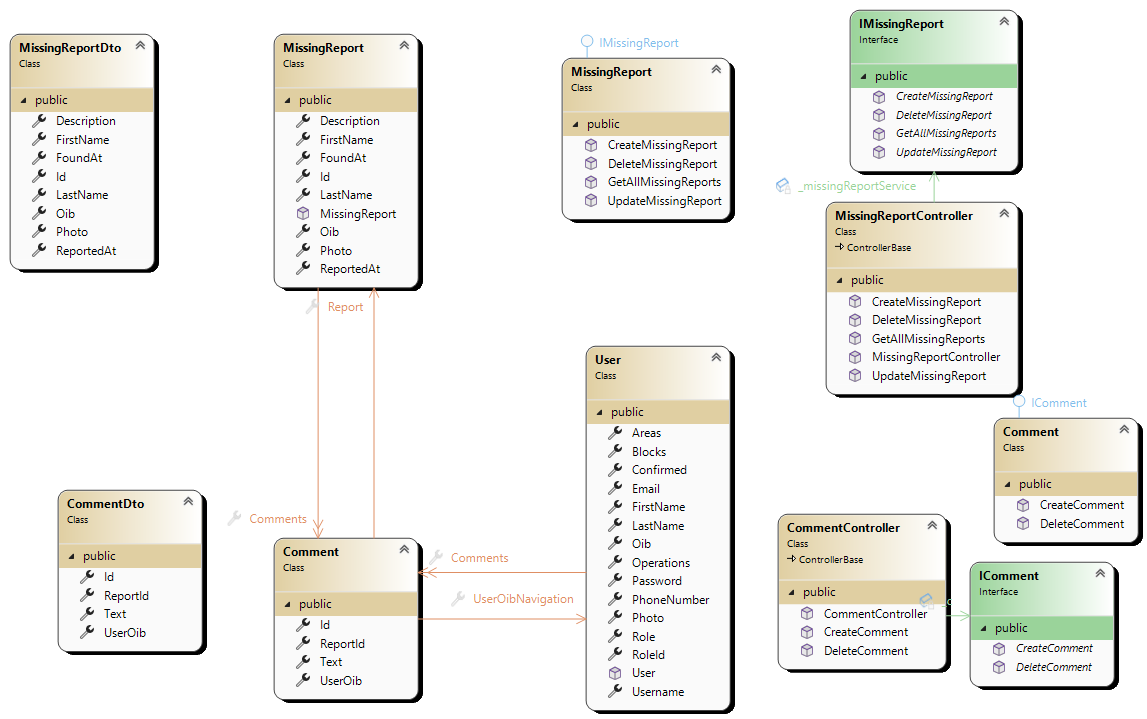
\includegraphics[width=\linewidth]{dijagrami/CD-CommentMissingReport.png}
				\caption{Dijagram razreda 2 - Missing Report i Comment}
			\end{figure}
		
		\eject
		
		Ovaj dijagram prikazuje razrede vezane za mapu, operacije i područja te kao takav čini ključni dio aplikacije. Iz ovog dijagrama razvidna je hijerarhija svih područja. Controlleri OperationController, MapController, BlockController i BuildingController nasljeđuju metode za stvaranje operacija i područja, kao i za mijenjanje njihova statusa. Modeli operacije, regije, blokovi i zgrade međusobno su povezani relacijama generalizacija i pridruživanje. Modeli i DTO-ovi također su povezani s Userom relacijama pridruživanja te su prikazane operacije, područja i blokovi povezani s tim Userom.
		
			\begin{figure}[h!] 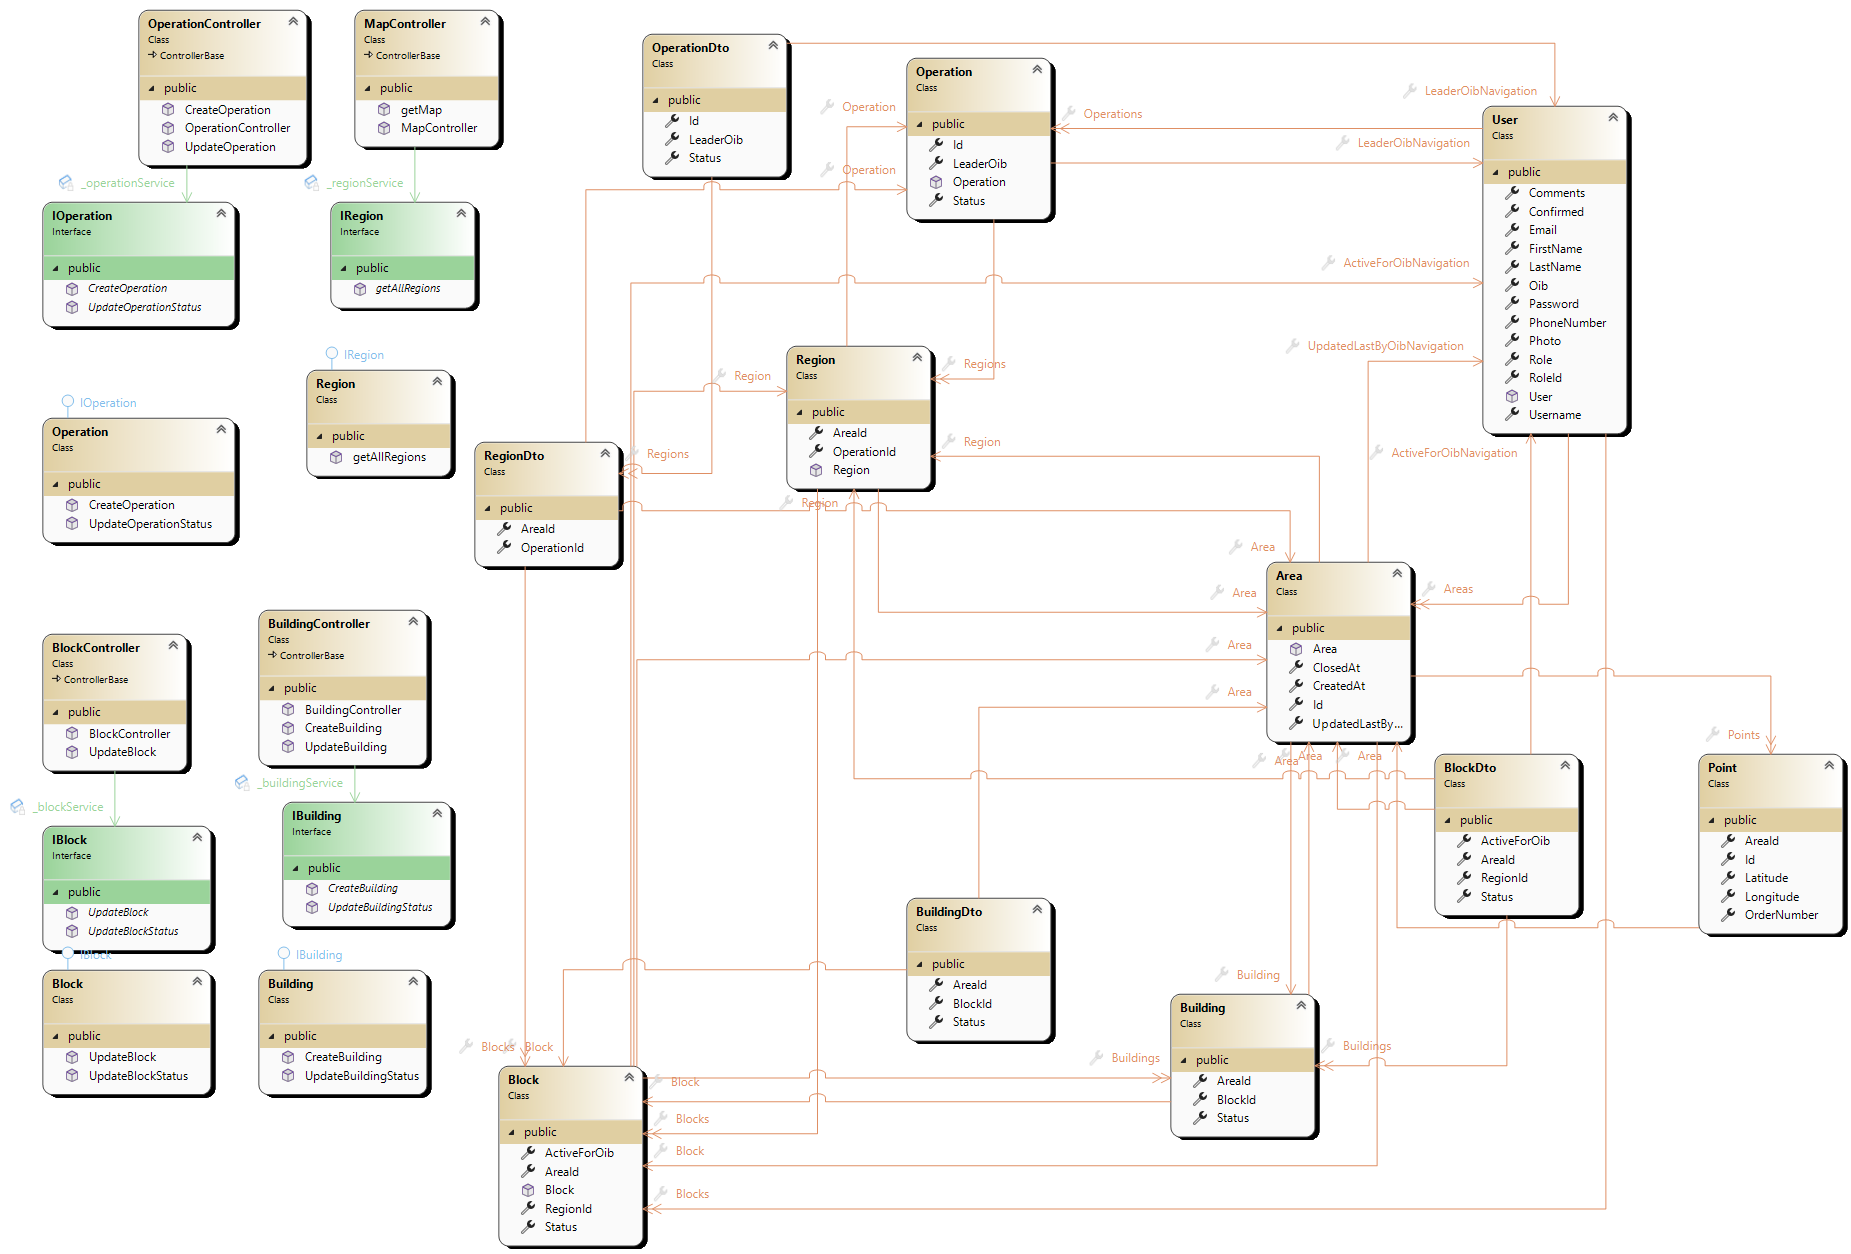
\includegraphics[width=\linewidth]{dijagrami/CD-AreasOperations.png}
				\caption{Dijagram razreda 3 - Operations, Areas, Regions, Blocks, Buildings}
			\end{figure}
		
		\eject
		
		Na slici 4.7 prikazani su Controlleri, Modeli i Servicei User i Role. UserController implementira IServiceUser te implementira metode za potvrdu, brisanje, dohvat, ažuriranje te dohvat svih korisnika. Modeli User i Role također su međusobno povezani pridruživanjem. Vidimo i da se podaci o Useru spremaju u bazu podataka.
		
			\begin{figure}[h!] 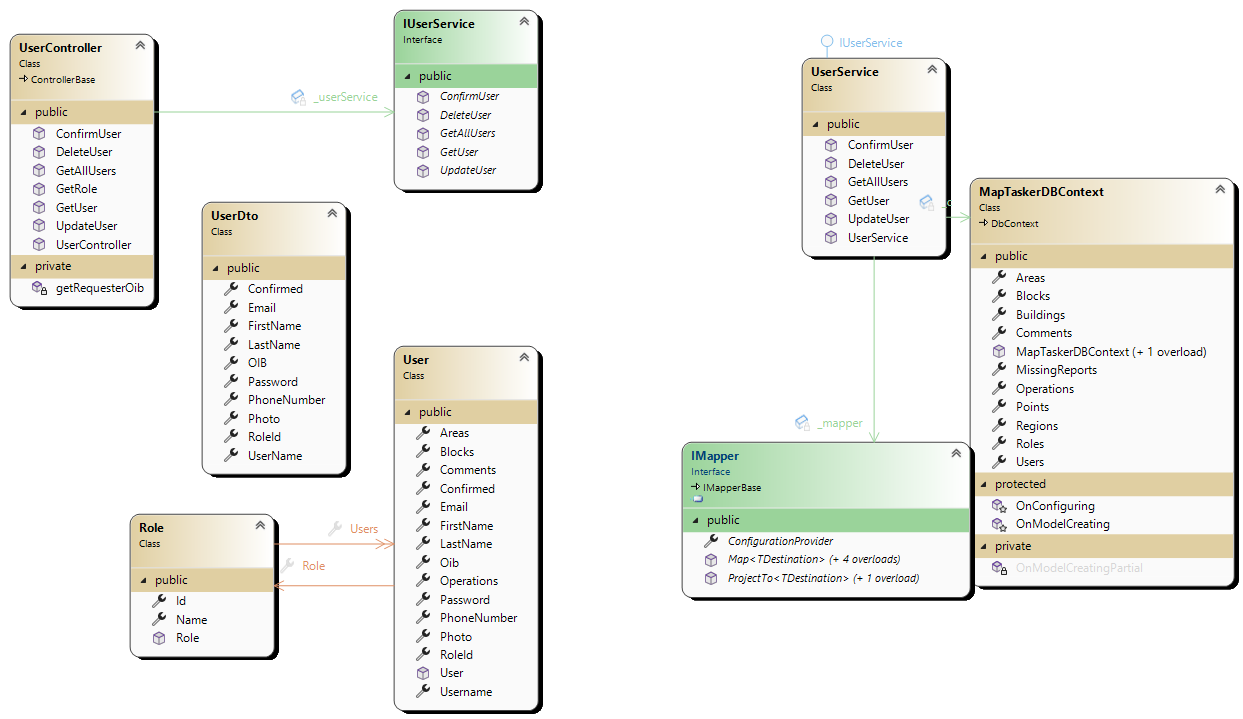
\includegraphics[width=\linewidth]{dijagrami/CD-UserRole.png}
				\caption{Dijagram razreda 4 - User i Role}
			\end{figure}
		
		\eject
		
		Na slici 4.8 nalazi se dijagram koji prikazuje statistiku. StatisticsController realizira sučelje IStatistic te njegovu metodu getStatistic za dohvat statistike. Data transfer object StatisticDto povezan je s DTO-ovima MissingReport, Block i Building kako bi mogao prikazati potrebne podatke.
		
			\begin{figure}[h!] 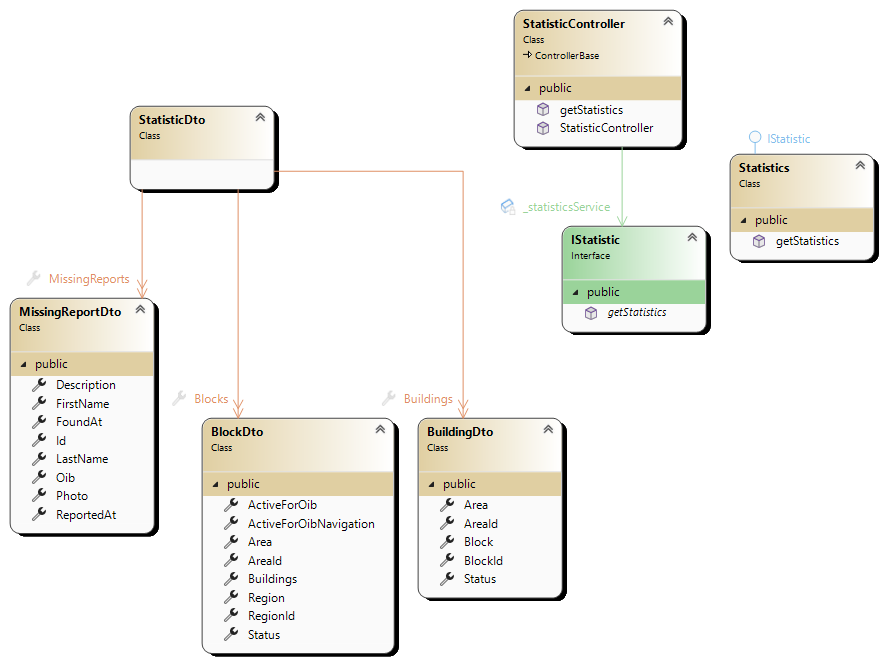
\includegraphics[width=\linewidth]{dijagrami/CD-Statistics.png}
				\caption{Dijagram razreda 5 - Statistics}
			\end{figure}
					
		\eject
		
		\section{Dijagram stanja}
			
			
			\textbf{\textit{dio 2. revizije}}\\
			
			\textit{Potrebno je priložiti dijagram stanja i opisati ga. Dovoljan je jedan dijagram stanja koji prikazuje \textbf{značajan dio funkcionalnosti} sustava. Na primjer, stanja korisničkog sučelja i tijek korištenja neke ključne funkcionalnosti jesu značajan dio sustava, a registracija i prijava nisu. }
			
			
			\eject 
		
		\section{Dijagram aktivnosti}
			
			\textbf{\textit{dio 2. revizije}}\\
			
			 \textit{Potrebno je priložiti dijagram aktivnosti s pripadajućim opisom. Dijagram aktivnosti treba prikazivati značajan dio sustava.}
			
			\eject
		\section{Dijagram komponenti}
		
			\par
			Ovaj dijagram pokazuje organizaciju i međuodnos komponenti, unutarnje strukture te odnos prema okolini. Postoje 3 vrste sučelja: za dohvat CSS, JS i TSX datoteka, za dohvat JSON podataka kojim se pristupa REST API komponenti te za dohvat tablica iz baze podataka. Preko glavne komponente App pristupa se ostalim komponentama. Preko drugog sučelja za dohvat JSON-a pristupa se Rest API-ju koji zatim poslužuje podatke koji pripadaju \textit{backend} dijelu aplikacije. Tablice se iz baze podataka dohvaćaju preko sučelja za dohvat podataka iz baze te se šalju u obliku DTO-a MVC arhitekturi na daljnju manipulaciju.
			
			\begin{figure}[H] 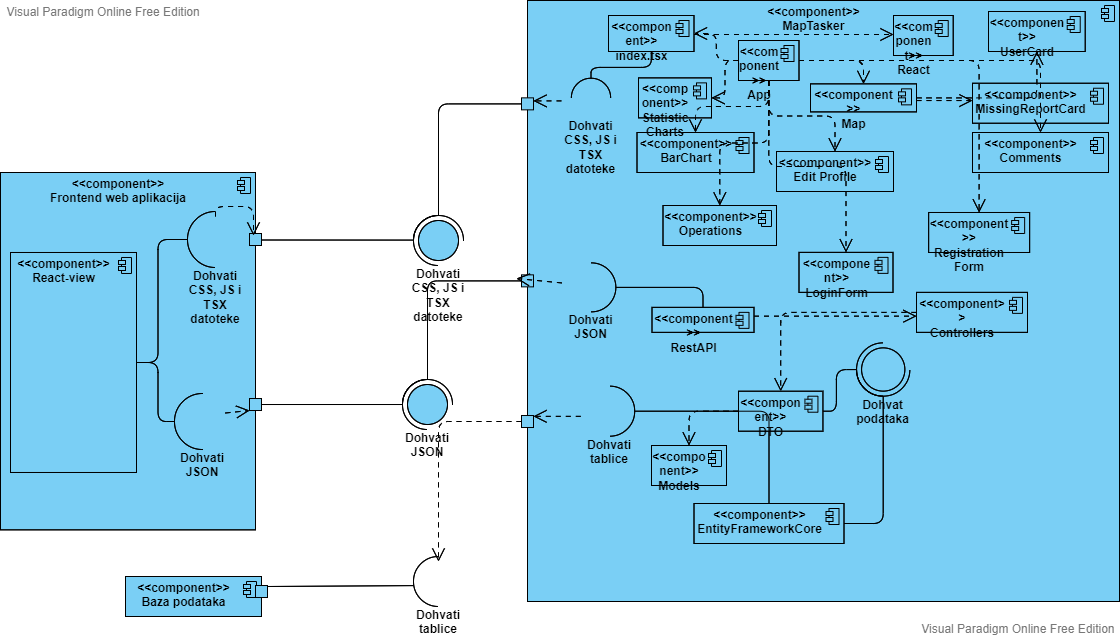
\includegraphics[width=\linewidth]{./dijagrami/ComponentDiagram.vpd.png}
				\caption{Dijagram komponenti}
			\end{figure}
		
		\eject

	


\chapter{Implementacija i korisničko sučelje}
		
		
		\section{Korištene tehnologije i alati}
			 
			 \par
			 Komunikacija u timu realizirana je korištenjem aplikacija \underline{WhatsApp}\footnote{\url{https://www.whatsapp.com/}} i \underline{Discord}\footnote{\url{https://discord.com/}}. Za izradu UML dijagrama korišten je alat \underline{Visual Paradigm Online}\footnote{\url{https://online.visual-paradigm.com/}}. Kao sustav za upravljanje izvornim kodom korišten je \underline{Git}\footnote{\url{https://git-scm.com/}} te je udaljeni repozitorij projekta dostupan na platformi \underline{GitLab}\footnote{\url{https://gitlab.com/}}. Za izradu dokumentacije korišten je softverski sustav za pripremu dokumenata \underline{LaTeX}\footnote{\url{https://www.latex-project.org/}}.
			 \par
			 Kao razvojno okruženje korišteno je integrirano razvojno okruženje Microsofta - \underline{Microsoft Visual Studio}\footnote{\url{https://visualstudio.microsoft.com/}}. Čini ga opsežan skup alata za izgradnju ASP.NET aplikacija, desktop aplikacija i mobilnih aplikacija. Kao urednik izvornog koda za rad na \textit{frontendu} korišten je i Microsoftov uređivač izvornog koda - \underline{Visual Studio Code}\footnote{\url{https://code.visualstudio.com/}}.
			 \par
			 Za izradu \textit{frontend} dijela aplikacije korišten je \underline{.NET Framework}\footnote{\url{https://dotnet.microsoft.com}} te \underline{C sharp}\footnote{\url{https://https://docs.microsoft.com/en-us/dotnet/csharp/}}, dok je \textit{backend} dio aplikacije napravljen koristeći \underline{React}\footnote{\url{https://https://reactjs.org/}} i \underline{JavaScript}\footnote{\url{https://https://www.javascript.com/}}. .Net Framework jest radni okvir razvijen od strane Microsofta koji programerima uvelike pomaže u prevođenju i izvođenju programa. React je besplatna JavaScript biblioteka otvorenog koda za izgradnju korisničkih sučelja.
			 \par
			 Baza podataka nalazi se na poslužitelju u oblaku \underline{Microsoft Azureu}\footnote{\url{https://portal.azure.com/}}. To je računalna platforma koja omogućuje pristup i upravljanje aplikacijama i uslugama. 
			
			\eject 
		
	
		\section{Ispitivanje programskog rješenja}
			
			\subsection{Ispitivanje komponenti}
			

			
			\par
			Svi unit testovi izvršeni su automatski. Ispitivanje je provedeno po serviceima te su se tako provjeravale pojedine komponente sustava. U svakom su testu na početku dohvaćeni DbContext i Mapper.
		
			
			\noindent \textbf{Ispitni slučaj 1: Dohvaćanje svih korisnika}
			
			\noindent \textbf{Ulaz:}
			
			\begin{packed_enum}
				
				\item Stvaranje novog UserServicea
				\item Dohvaćanje metode GetAllUsers
				
			\end{packed_enum}
		
			\noindent \textbf{Očekivani izlaz:}
		
			\begin{packed_enum}
			
				\item Stvara se novi UserService
				\item Dohvaćaju se svi korisnici
				\item Rezultat testa je ispravan
			
			\end{packed_enum}
		
			\noindent \textbf{Izlaz:} Test je zadovoljen. Aplikacija je prošla test.
			
			\begin{figure}[H] 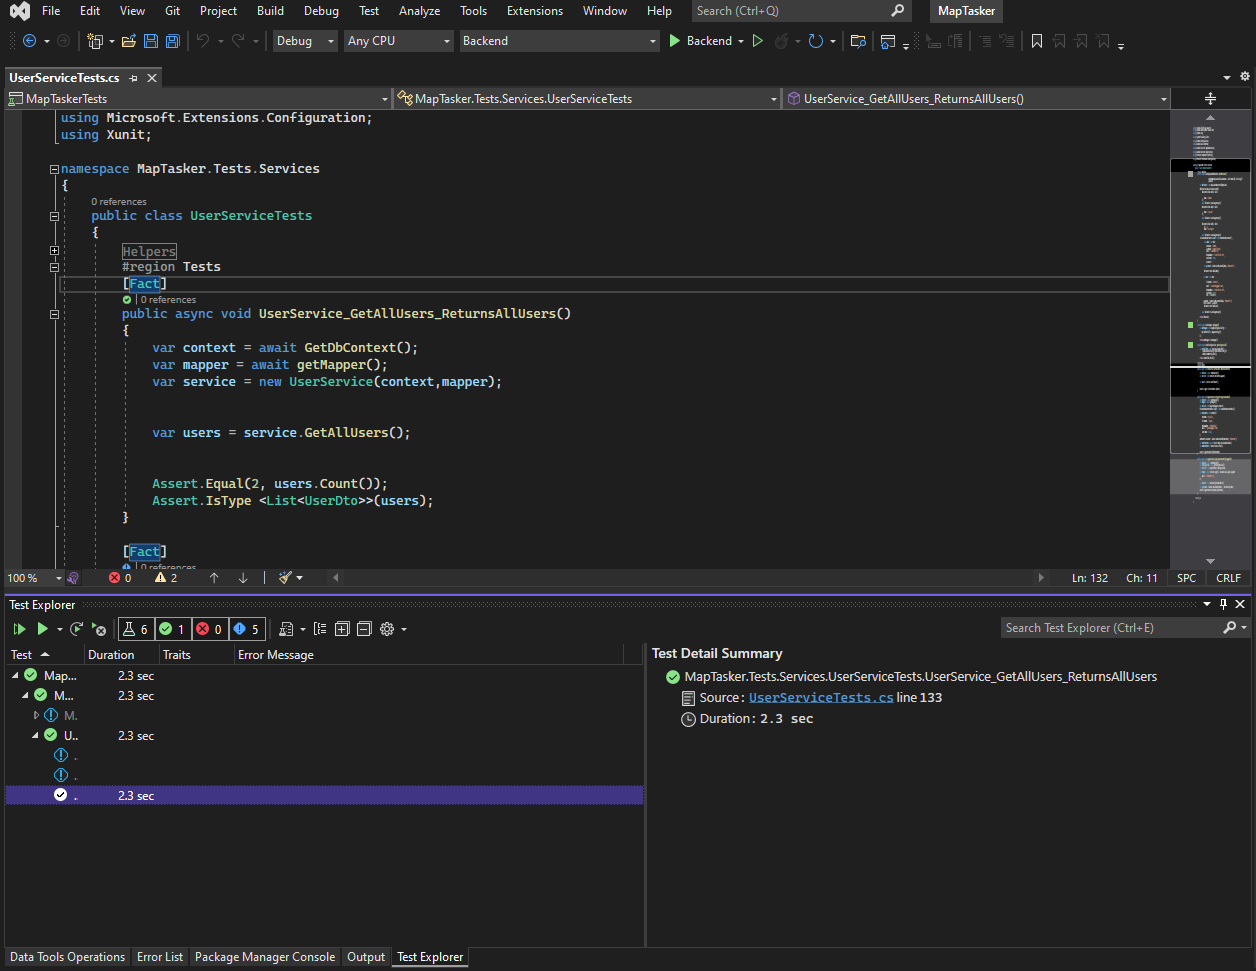
\includegraphics[width=\linewidth]{./slike/Testovi/Unit/UnitTest_1.png}
				\caption{GetAllUsers - ReturnsAllUsers Test}
			\end{figure}
			
			\eject
			
			\noindent \textbf{Ispitni slučaj 2: Uspješna registracija korisnika}
			
			\noindent \textbf{Ulaz:}
			
			\begin{packed_enum}
				
				\item Stvaranje novog RegisterServicea
				\item Kreiranje password hashera
				\item Instanciranje novog korisnika
				\item Postavljanje lozinke korisniku
				\item Dohvaćanje DTO-a Usera i ukupnog broja korisnika za provjeru
				
			\end{packed_enum}
			
			\noindent \textbf{Očekivani izlaz:}
			
			\begin{packed_enum}
				
				\item Stvara se novi RegisterService
				\item Kreira se novi password hasher
				\item Novi korisnik se uspješno stvara
				\item Lozinka se uspješno postavlja korisniku
				\item Rezultat testa je ispravan
				
			\end{packed_enum}
			
			\noindent \textbf{Izlaz:} Test je zadovoljen. Aplikacija je prošla test.
			
			\begin{figure}[H] 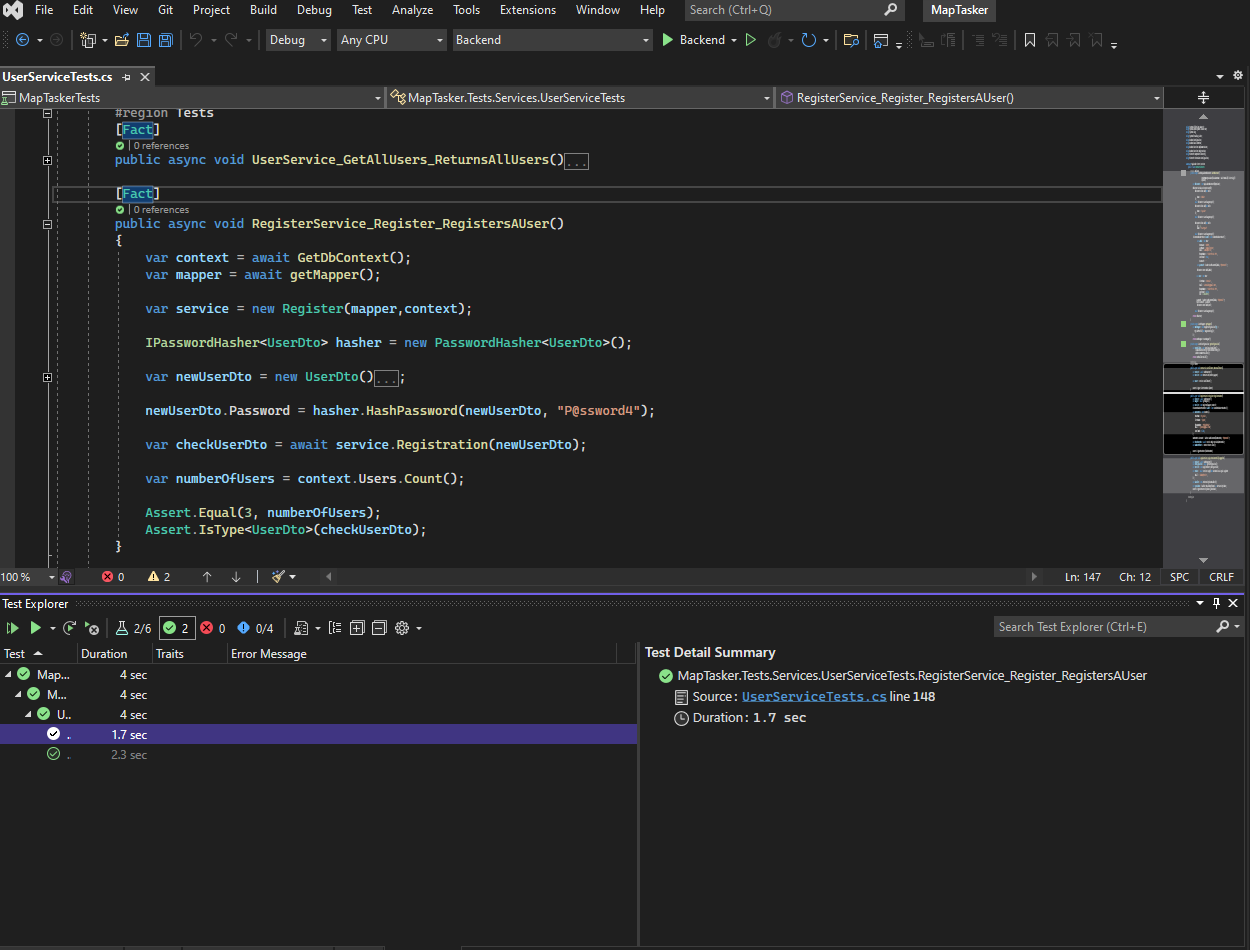
\includegraphics[width=\linewidth]{./slike/Testovi/Unit/UnitTest_2.png}
				\caption{Register - RegistersAnUser Test}
			\end{figure}
			
			\eject
		
			\noindent \textbf{Ispitni slučaj 3: Uspješna prijava korisnika}
			
			\noindent \textbf{Ulaz:}
			
			\begin{packed_enum}
				
				\item Stvaranje novog LoginServicea
				\item Kreiranje tokena koji se sastoji od e-mail adrese i lozinke
				\item Kreiranje handlera koji upravlja tokenima
				\item Dohvaćanje tokena
				
			\end{packed_enum}
			
			\noindent \textbf{Očekivani izlaz:}
			
			\begin{packed_enum}
				
				\item Stvara se novi LoginService
				\item Kreira se token za provjeru
				\item Kreira se handler koji upravlja tokenima
				\item Token se uspješno dohvaća
				\item Rezultat testa je ispravan
				
			\end{packed_enum}
			
			\noindent \textbf{Izlaz:} Test je zadovoljen. Aplikacija je prošla test.
			
			\begin{figure}[H] 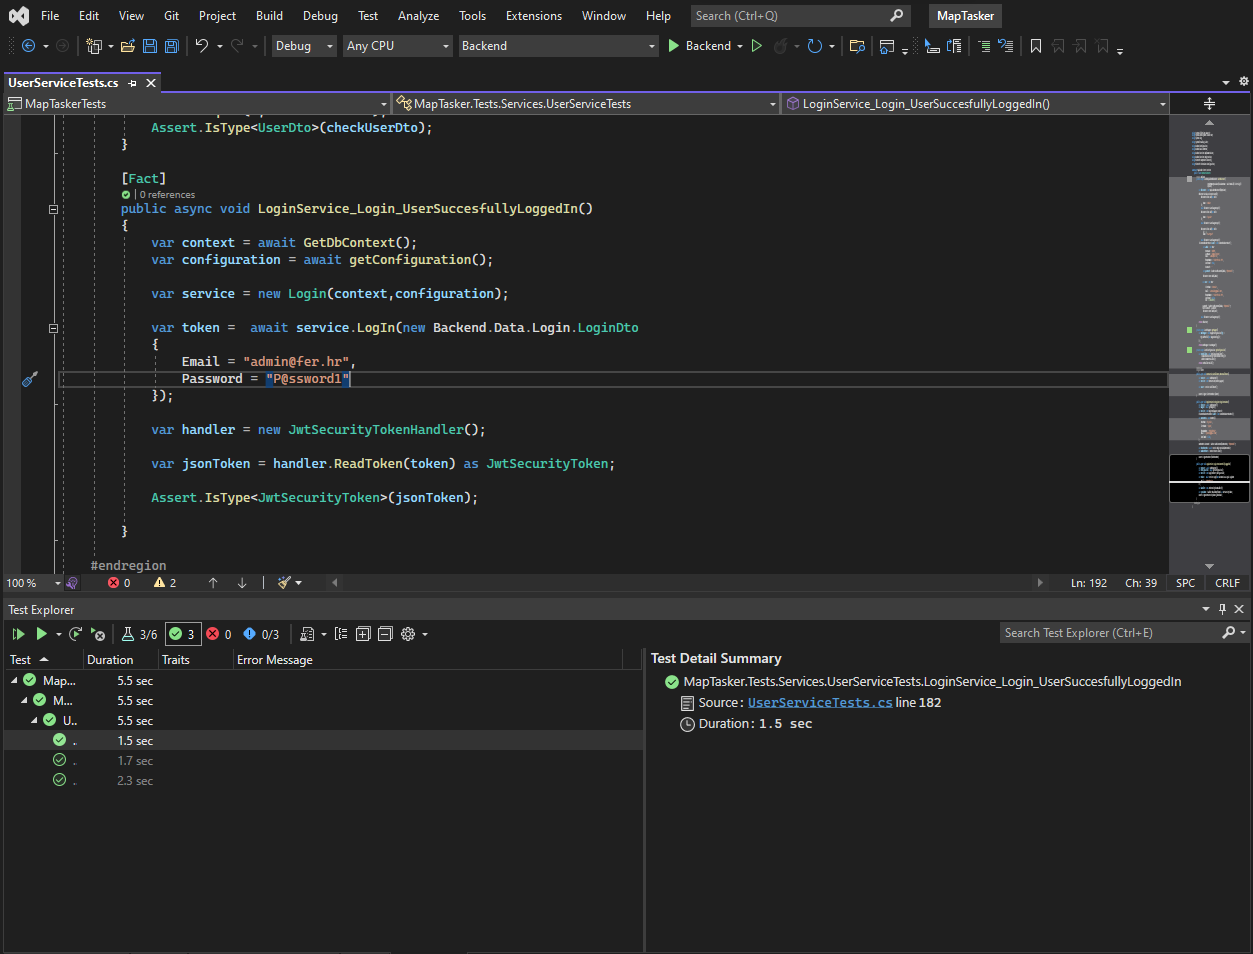
\includegraphics[width=\linewidth]{./slike/Testovi/Unit/UnitTest_3.png}
				\caption{UserSuccesfullyLoggedIn Test}
			\end{figure}
			
			\eject
			
			\noindent \textbf{Ispitni slučaj 4: Dohvaćanje svih prijava nestanka}
			
			\noindent \textbf{Ulaz:}
			
			\begin{packed_enum}
				
				\item Stvaranje novog generatora Id-a
				\item Kreiranje novog MissingReport Servicea
				\item Dohvaćanje svih prijava nestanaka metodom GetAllMissingReports
				
			\end{packed_enum}
			
			\noindent \textbf{Očekivani izlaz:}
			
			\begin{packed_enum}
				
				\item Stvara se generator Id-a
				\item Uspješno kreiranje MissingReporta
				\item Uspješno se dohvaćaju sve prijave nestanaka
				\item Rezultat testa je ispravan
				
			\end{packed_enum}
			
			\noindent \textbf{Izlaz:} Test je zadovoljen. Aplikacija je prošla test.
			
			\begin{figure}[H] 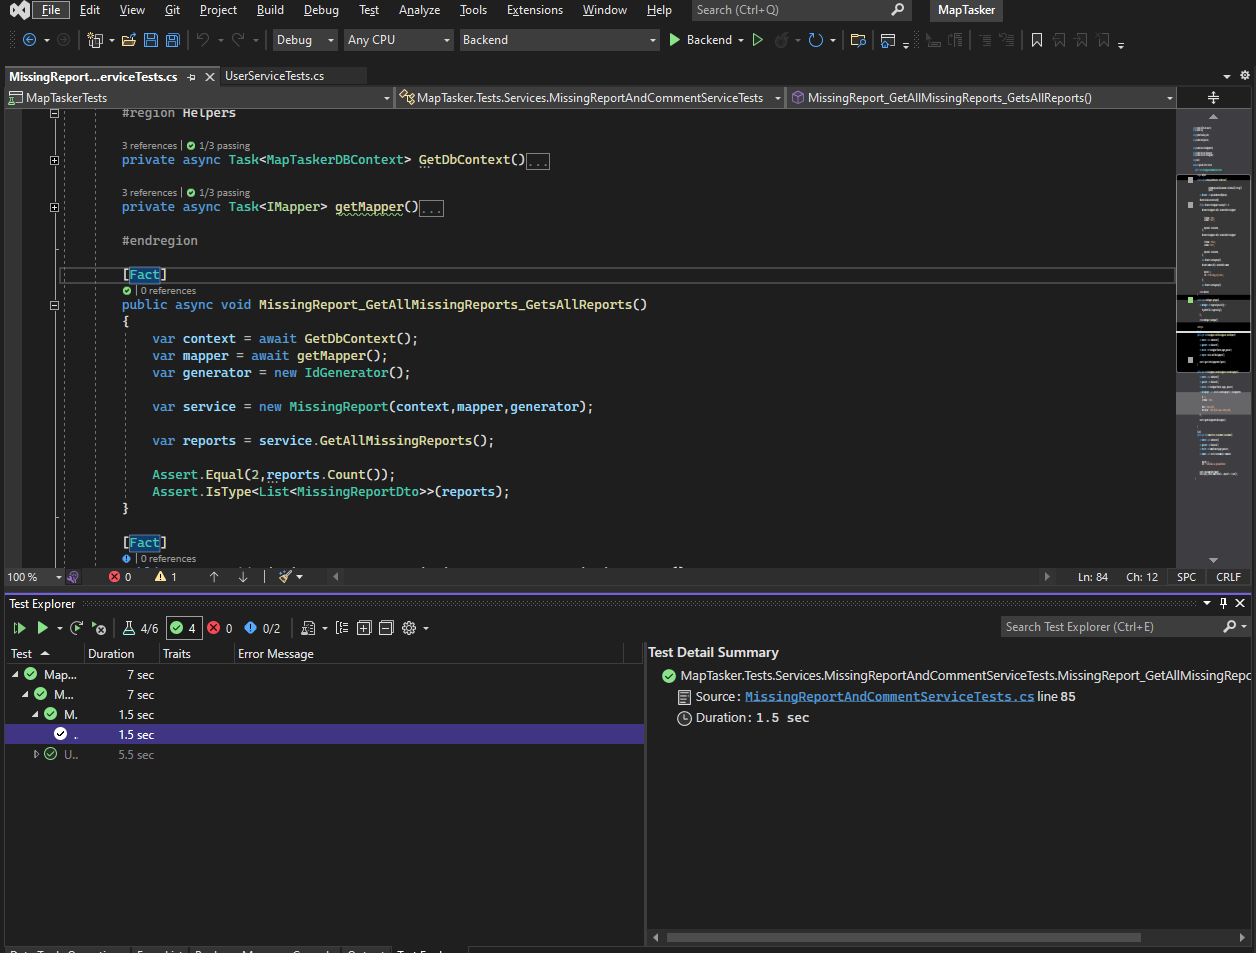
\includegraphics[width=\linewidth]{./slike/Testovi/Unit/UnitTest_4.png}
				\caption{GetAllMissingReports Test}
			\end{figure}
			
			\eject
			
			\noindent \textbf{Ispitni slučaj 5: Stvaranje prijave nestanka}
			
			\noindent \textbf{Ulaz:}
			
			\begin{packed_enum}
				
				\item Stvaranje novog generatora Id-a
				\item Kreiranje MissingReport Servicea
				\item Instanciranje prijave nestanka
				
			\end{packed_enum}
			
			\noindent \textbf{Očekivani izlaz:}
			
			\begin{packed_enum}
				
				\item Stvara se generator Id-a
				\item Uspješno kreiranje MissingReport Servicea
				\item Prijava nestanka uspješno je instancirana
				\item Rezultat testa je ispravan
				
			\end{packed_enum}
			
			\noindent \textbf{Izlaz:} Test je zadovoljen. Aplikacija je prošla test.
			
			\begin{figure}[H] 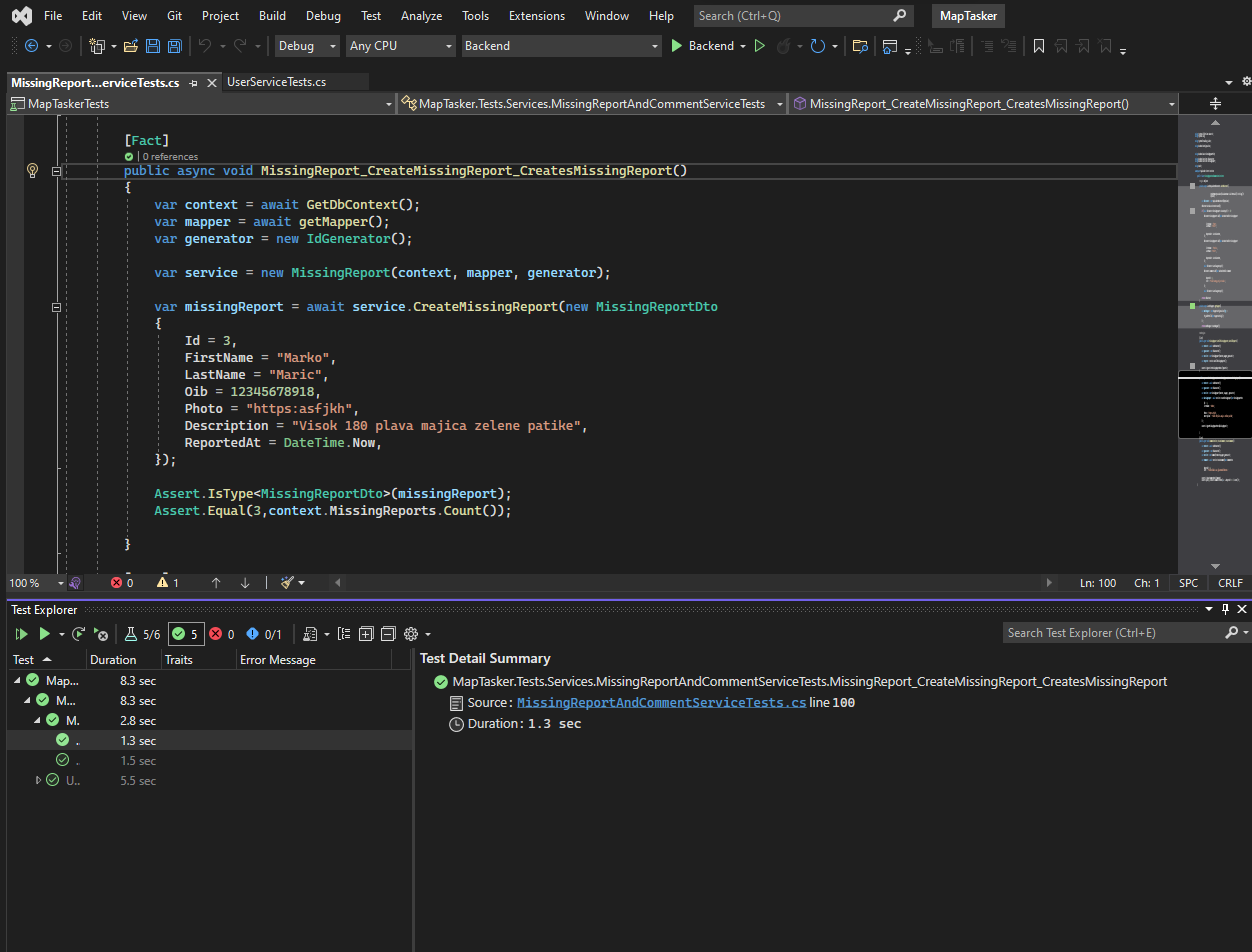
\includegraphics[width=\linewidth]{./slike/Testovi/Unit/UnitTest_5.png}
				\caption{CreatesMissingReport Test}
			\end{figure}
			
			\eject
			
			\noindent \textbf{Ispitni slučaj 6: Kreiranje komentara}
			
			\noindent \textbf{Ulaz:}
			
			\begin{packed_enum}
				
				\item Stvaranje novog generatora Id-a
				\item Kreiranje Comment Servicea
				\item Instanciranje novog komentara
				
			\end{packed_enum}
			
			\noindent \textbf{Očekivani izlaz:}
			
			\begin{packed_enum}
				
				\item Stvara se generator Id-a
				\item Uspješno se kreiran Comment Service
				\item Komentar je uspješno instanciran
				\item Rezultat testa je ispravan
				
			\end{packed_enum}
			
			\noindent \textbf{Izlaz:} Test je zadovoljen. Aplikacija je prošla test.
			
			\begin{figure}[H] 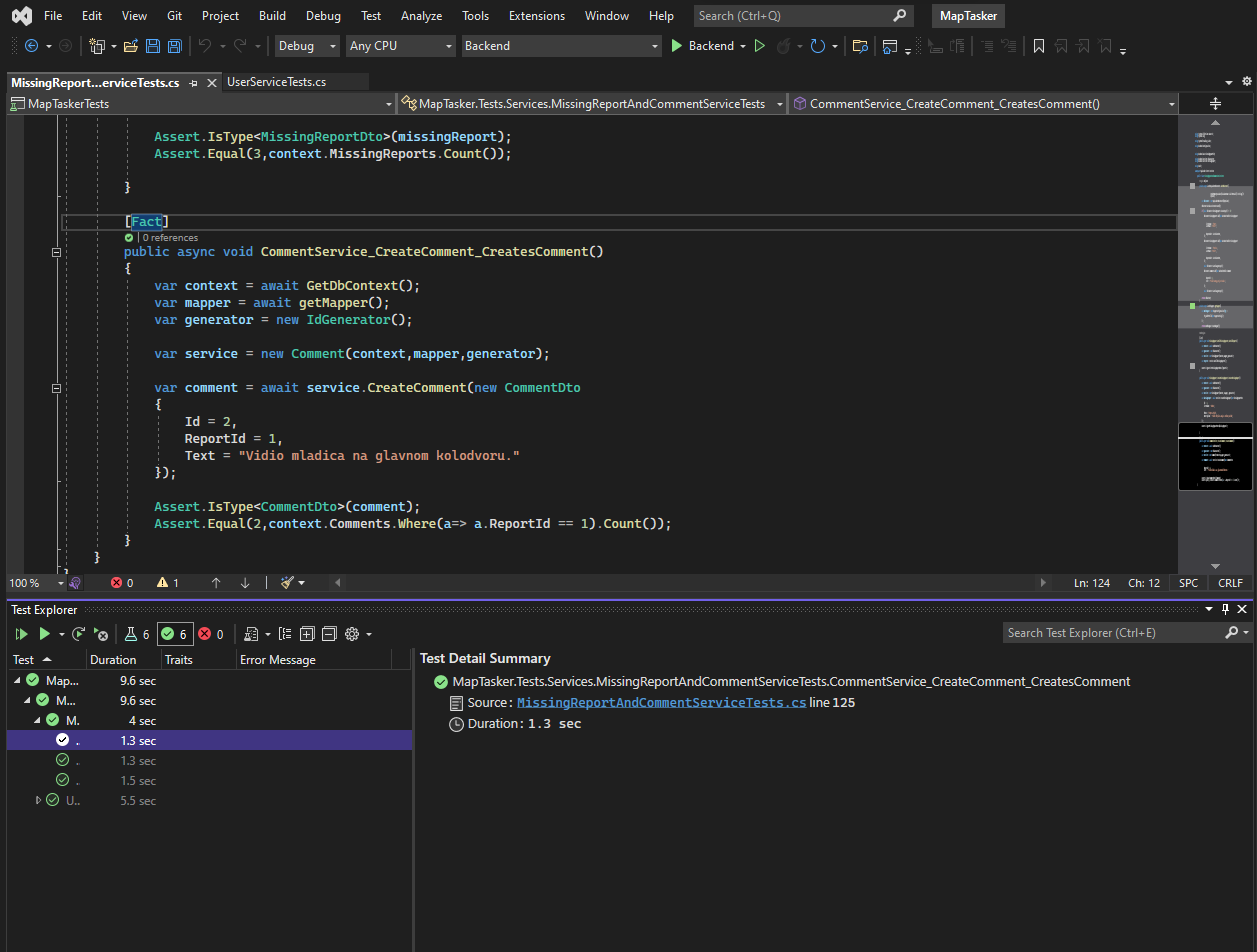
\includegraphics[width=\linewidth]{./slike/Testovi/Unit/UnitTest_6.png}
				\caption{CreatesComments Test}
			\end{figure}
			
			\eject
			
			
			
			\subsection{Ispitivanje sustava}
			
			\par
			Svi Selenium testovi izvršeni su automatski. Ispitivanje je provedeno po obrascima uporabe. Ispitani su obrasci uporabe:
			
			\begin{packed_enum}
				
				\item UC1 - Registracija u sustav
				\item UC2 - Prijava u sustav
				\item UC4 - Prijava nestale osobe
				\item UC5 - Komentiranje prijave nestale osobe
				
			\end{packed_enum}
		
			
			\noindent \textbf{Ispitni slučaj 1: Registracija}
			
			\noindent \textbf{Ulaz:}
			
			\begin{packed_enum}
				
				\item Učitavanje početne stranice i namještanje veličine prozora
				\item Pritisak na gumb "Register"
				\item Korisnik unosi tražene podatke te odabire ulogu koju želi
				
			\end{packed_enum}
			
			\noindent \textbf{Očekivani izlaz:}
			
			\begin{packed_enum}
				
				\item Početna stranica uspješno se učitava
				\item Učitavanje forme za registraciju
				\item Korisnik prima obavijest o uspješno obavljenoj registraciji
				\item Rezultat testa je ispravan
				
			\end{packed_enum}
			
			\noindent \textbf{Izlaz:} Test je zadovoljen. Aplikacija je prošla test.
			
			\begin{figure}[H] 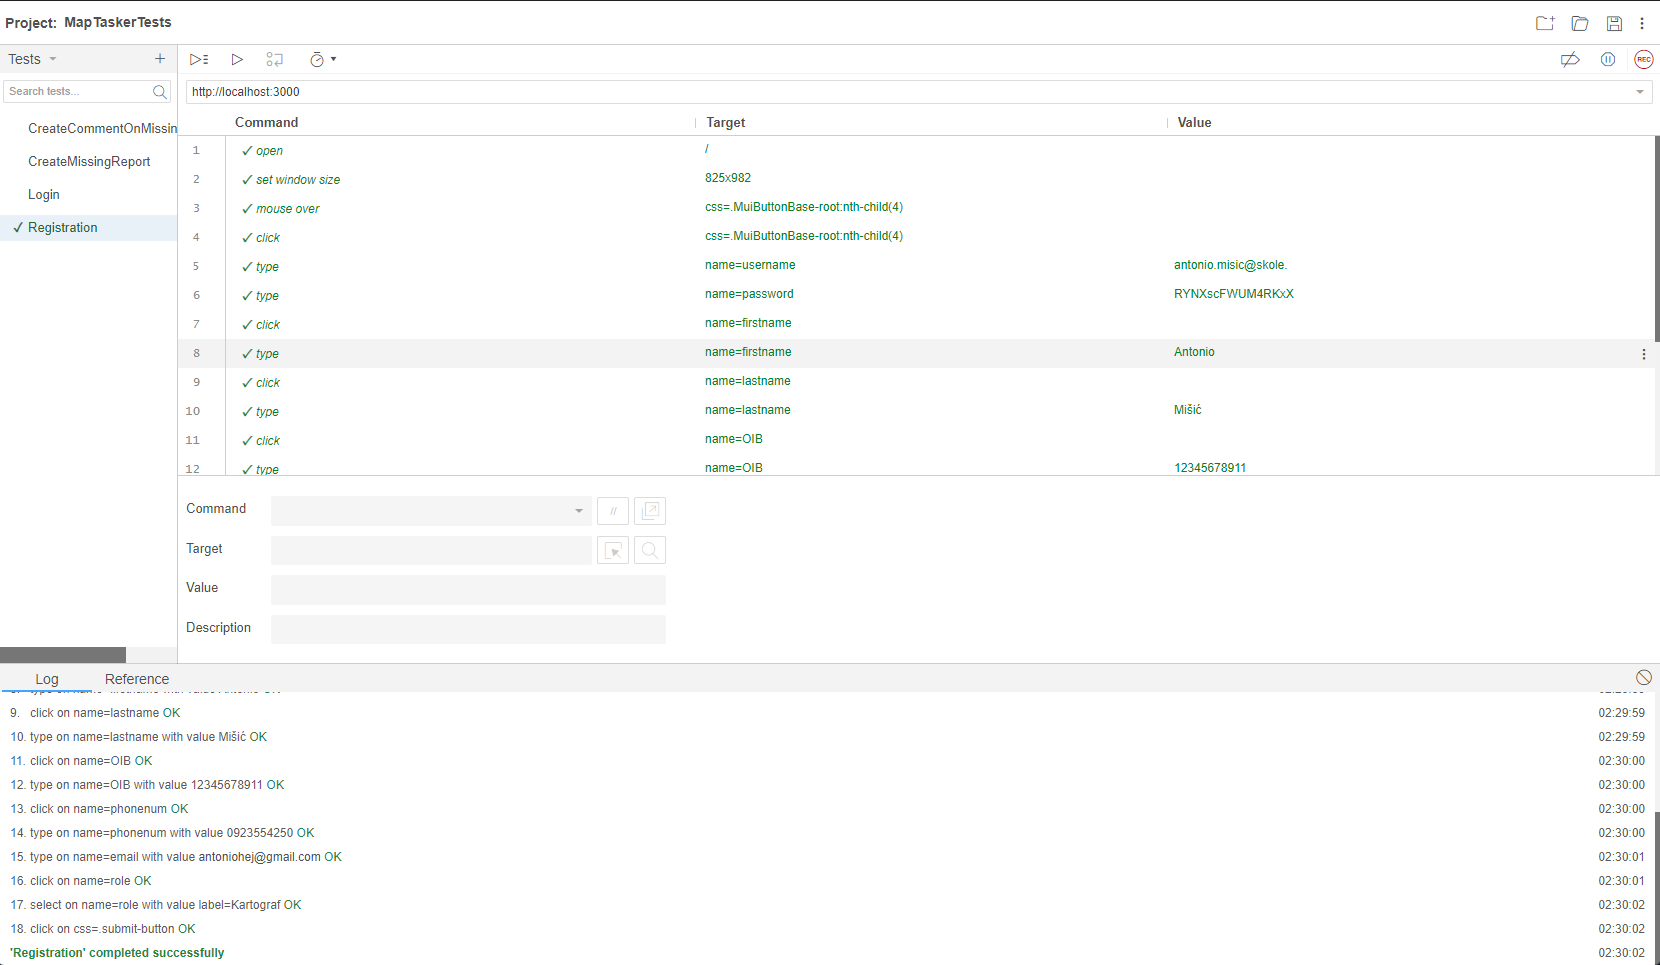
\includegraphics[width=\linewidth]{./slike/Testovi/Selenium/Selenium_1.png}
				\caption{Registration Test}
			\end{figure}
			
			\eject
			
			\noindent \textbf{Ispitni slučaj 2: Prijava}
			
			\noindent \textbf{Ulaz:}
			
			\begin{packed_enum}
				
				\item Učitavanje početne stranice i namještanje veličine prozora
				\item Pritisak na gumb "Login"
				\item Korisnik unosi e-mail adresu i lozinku
				
			\end{packed_enum}
			
			\noindent \textbf{Očekivani izlaz:}
			
			\begin{packed_enum}
				
				\item Početna stranica uspješno se učitava
				\item Učitavanje forme za prijavu
				\item Korisnik je uspješno prijavljen u sustav
				\item Rezultat testa je ispravan
				
			\end{packed_enum}
			
			\noindent \textbf{Izlaz:} Test je zadovoljen. Aplikacija je prošla test.
			
			\begin{figure}[H] 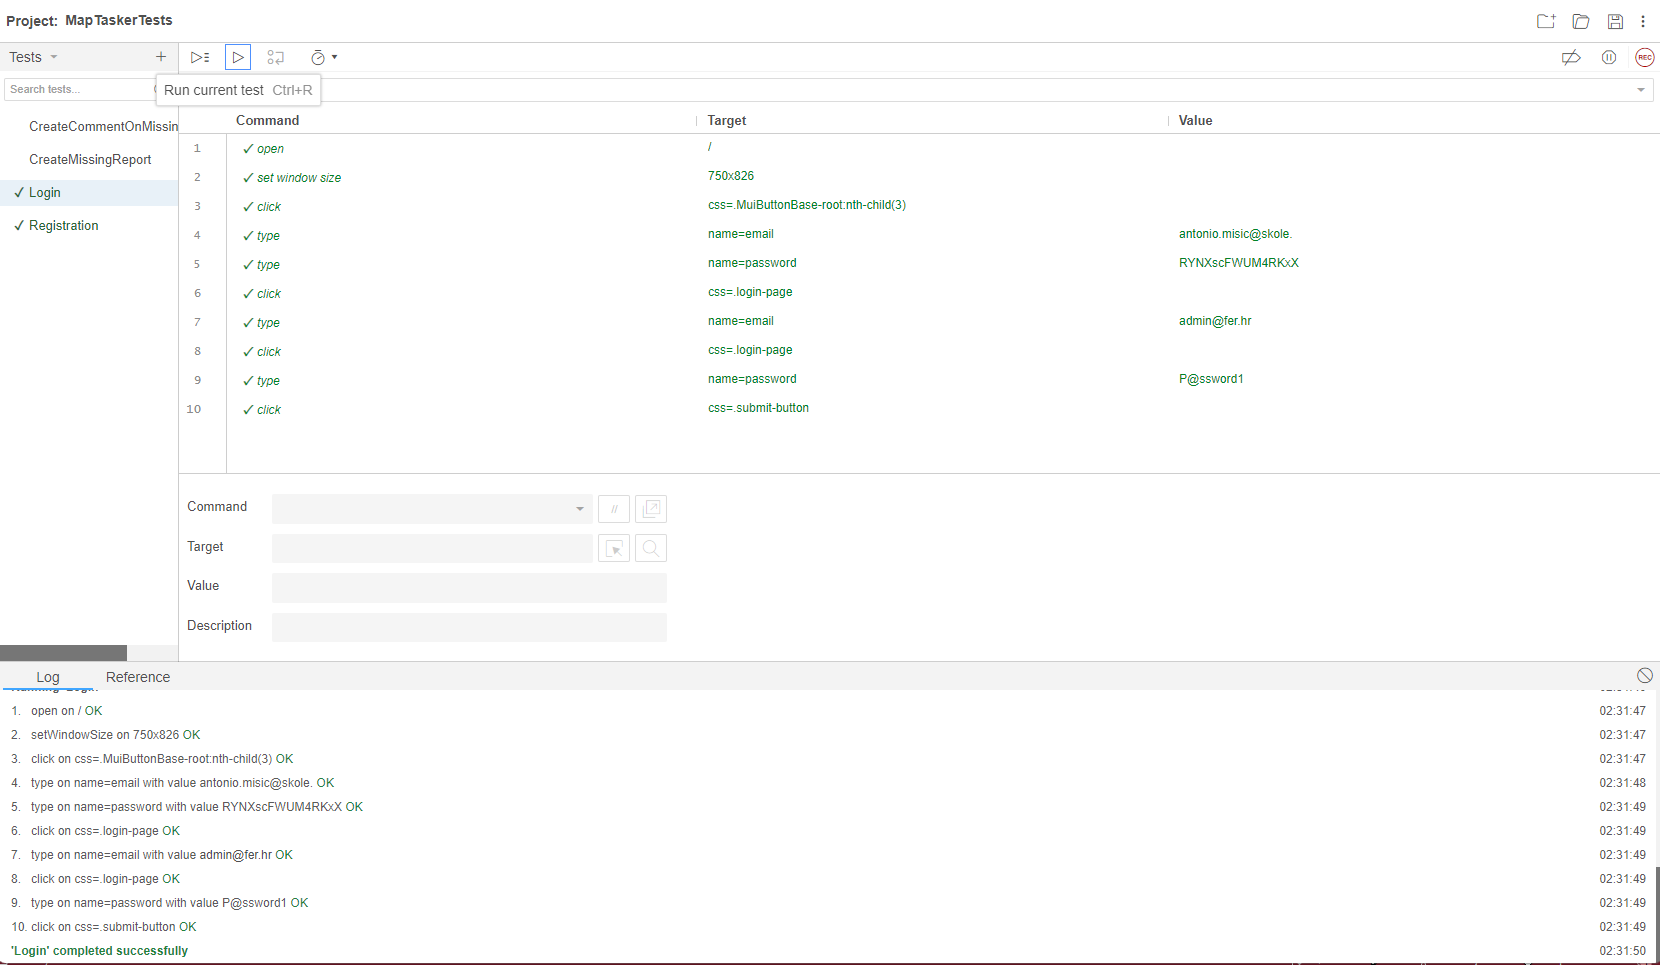
\includegraphics[width=\linewidth]{./slike/Testovi/Selenium/Selenium_2.png}
				\caption{Login Test}
			\end{figure}
			
			\eject
			
			\noindent \textbf{Ispitni slučaj 3: Kreiranje prijave nestanka}
			
			\noindent \textbf{Ulaz:}
			
			\begin{packed_enum}
				
				\item Učitavanje početne stranice i namještanje veličine prozora
				\item Pritisak na gumb "Prijavi"
				\item Unošenje podataka o nestaloj osobi
				
			\end{packed_enum}
			
			\noindent \textbf{Očekivani izlaz:}
			
			\begin{packed_enum}
				
				\item Početna stranica uspješno se učitava
				\item Učitavanje forme za prijavu nestanka osobe
				\item Obavijest o uspješnoj prijavi nestale osobe
				\item Rezultat testa je ispravan
				
			\end{packed_enum}
			
			\noindent \textbf{Izlaz:} Test je zadovoljen. Aplikacija je prošla test.
			
			\begin{figure}[H] 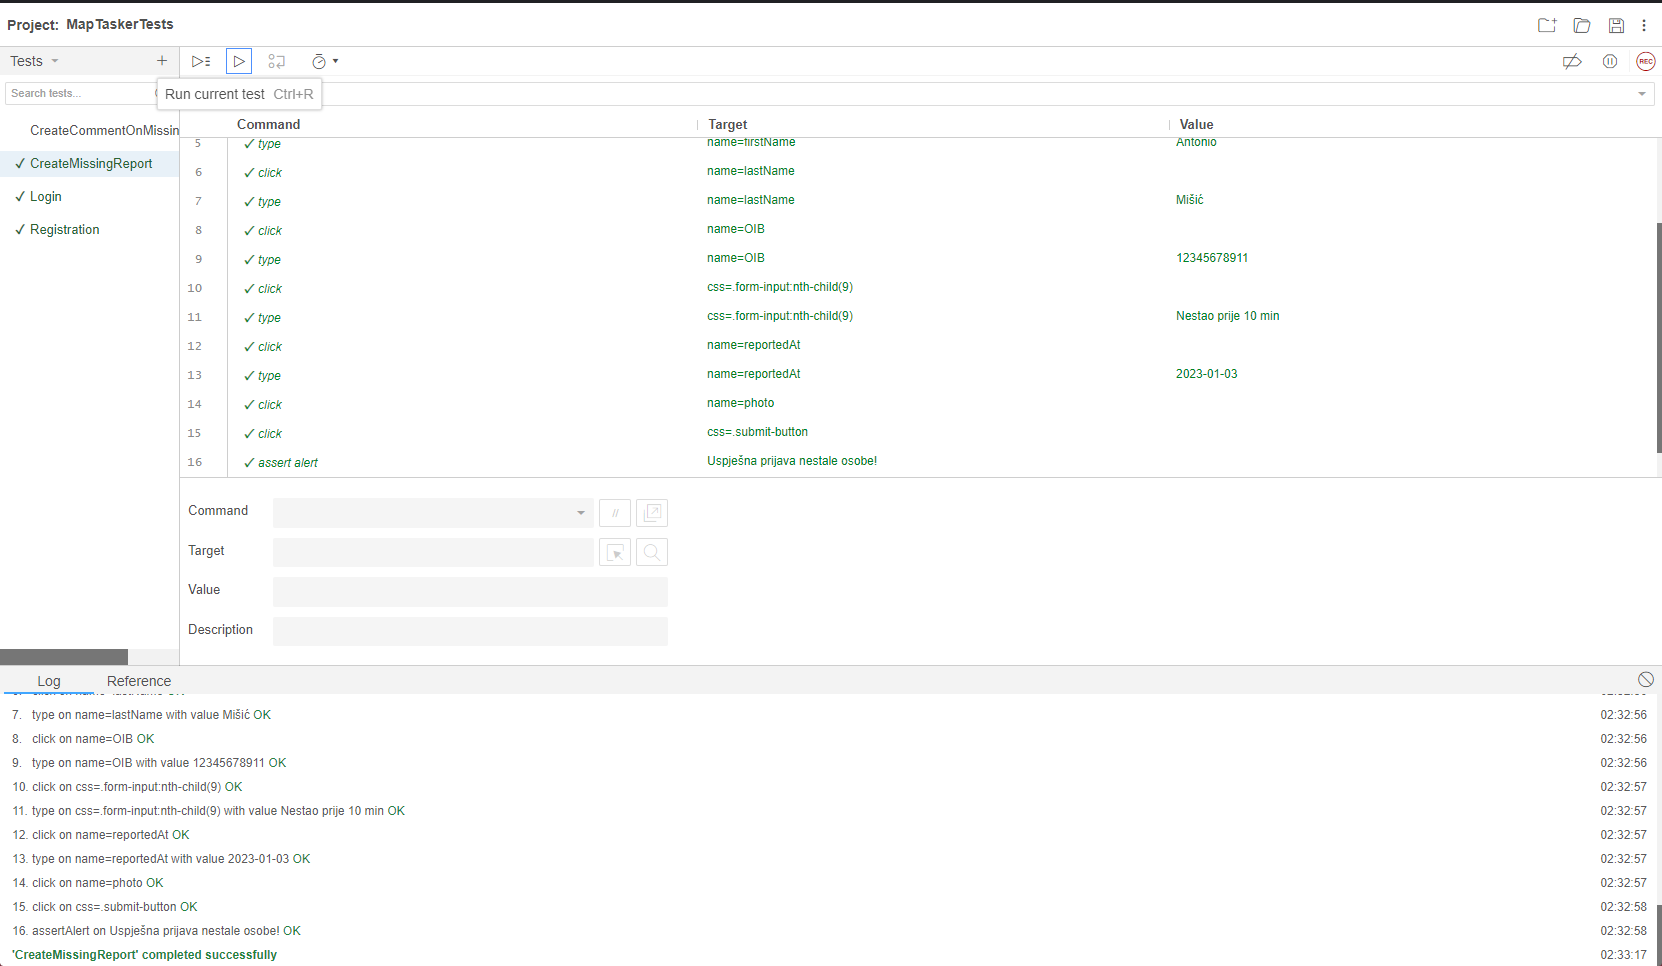
\includegraphics[width=\linewidth]{./slike/Testovi/Selenium/Selenium_3.png}
				\caption{CreateMissingReport Test}
			\end{figure}
			
			\eject
			
			\noindent \textbf{Ispitni slučaj 4: Kreiranje komentara na prijavu nestanka}
			
			\noindent \textbf{Ulaz:}
			
			\begin{packed_enum}
				
				\item Učitavanje početne stranice i namještanje veličine prozora
				\item Pritisak na gumb "Nestale osobe"
				\item Stvaranje komentara kraj nestale osobe
				
			\end{packed_enum}
			
			\noindent \textbf{Očekivani izlaz:}
			
			\begin{packed_enum}
				
				\item Početna stranica uspješno se učitava
				\item Učitavanje stranice s nestalim osobama
				\item Komentar je prikazan na stranici
				\item Rezultat testa je ispravan
				
			\end{packed_enum}
			
			\noindent \textbf{Izlaz:} Test je zadovoljen. Aplikacija je prošla test.
			
			\begin{figure}[H] 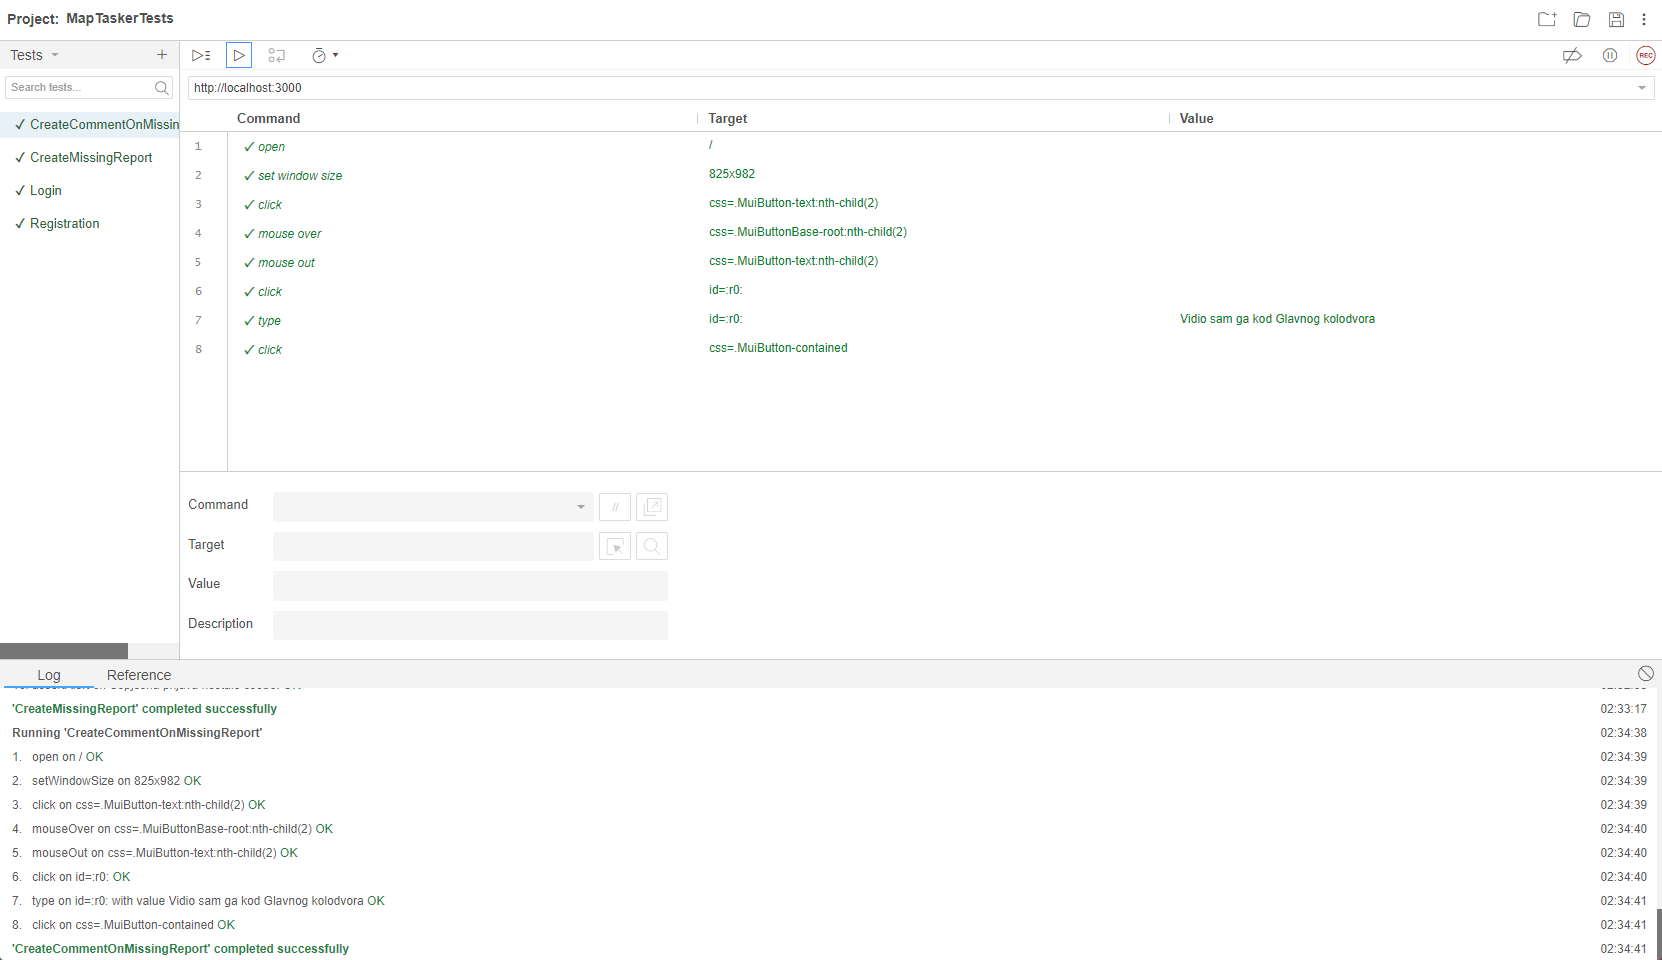
\includegraphics[width=\linewidth]{./slike/Testovi/Selenium/Selenium_4.png}
				\caption{CreateComment Test}
			\end{figure}
			
			\eject
		
		
		\section{Dijagram razmještaja}
			
			\textbf{\textit{dio 2. revizije}}
			
			 \textit{Potrebno je umetnuti \textbf{specifikacijski} dijagram razmještaja i opisati ga. Moguće je umjesto specifikacijskog dijagrama razmještaja umetnuti dijagram razmještaja instanci, pod uvjetom da taj dijagram bolje opisuje neki važniji dio sustava.}
			
			\eject 
		
		\section{Upute za puštanje u pogon}
		
			\textbf{\textit{dio 2. revizije}}\\
		
			 \textit{U ovom poglavlju potrebno je dati upute za puštanje u pogon (engl. deployment) ostvarene aplikacije. Na primjer, za web aplikacije, opisati postupak kojim se od izvornog kôda dolazi do potpuno postavljene baze podataka i poslužitelja koji odgovara na upite korisnika. Za mobilnu aplikaciju, postupak kojim se aplikacija izgradi, te postavi na neku od trgovina. Za stolnu (engl. desktop) aplikaciju, postupak kojim se aplikacija instalira na računalo. Ukoliko mobilne i stolne aplikacije komuniciraju s poslužiteljem i/ili bazom podataka, opisati i postupak njihovog postavljanja. Pri izradi uputa preporučuje se \textbf{naglasiti korake instalacije uporabom natuknica} te koristiti što je više moguće \textbf{slike ekrana} (engl. screenshots) kako bi upute bile jasne i jednostavne za slijediti.}
			
			
			 \textit{Dovršenu aplikaciju potrebno je pokrenuti na javno dostupnom poslužitelju. Studentima se preporuča korištenje neke od sljedećih besplatnih usluga: \href{https://aws.amazon.com/}{Amazon AWS}, \href{https://azure.microsoft.com/en-us/}{Microsoft Azure} ili \href{https://www.heroku.com/}{Heroku}. Mobilne aplikacije trebaju biti objavljene na F-Droid, Google Play ili Amazon App trgovini.}
			
			
			\eject 


	\begin{comment}

\chapter{Zaključak i budući rad}
		
		\textbf{\textit{dio 2. revizije}}\\
		
		 \textit{U ovom poglavlju potrebno je napisati osvrt na vrijeme izrade projektnog zadatka, koji su tehnički izazovi prepoznati, jesu li riješeni ili kako bi mogli biti riješeni, koja su znanja stečena pri izradi projekta, koja bi znanja bila posebno potrebna za brže i kvalitetnije ostvarenje projekta i koje bi bile perspektive za nastavak rada u projektnoj grupi.}
		
		 \textit{Potrebno je točno popisati funkcionalnosti koje nisu implementirane u ostvarenoj aplikaciji.}
		
		\eject 

\end{comment}

	\chapter*{Popis literature}
		\addcontentsline{toc}{chapter}{Popis literature}
	 	
 		\textbf{\textit{Kontinuirano osvježavanje}}
	
		\textit{Popisati sve reference i literaturu koja je pomogla pri ostvarivanju projekta.}
		
		
		\begin{enumerate}
			
			
			\item  Programsko inženjerstvo, FER ZEMRIS, \url{http://www.fer.hr/predmet/proinz}
			
			\item  I. Sommerville, "Software engineering", 8th ed, Addison Wesley, 2007.
			
			\item  T.C.Lethbridge, R.Langaniere, "Object-Oriented Software Engineering", 2nd ed. McGraw-Hill, 2005.
			
			\item  I. Marsic, Software engineering book``, Department of Electrical and Computer Engineering, Rutgers University, \url{http://www.ece.rutgers.edu/~marsic/books/SE}
			
			\item  The Unified Modeling Language, \url{https://www.uml-diagrams.org/}
			
			\item  Astah Community, \url{http://astah.net/editions/uml-new}
		\end{enumerate}
		
		 
	
	
	\begingroup
	\renewcommand*\listfigurename{Indeks slika i dijagrama}
	%\renewcommand*\listtablename{Indeks tablica}
	%\let\clearpage\relax
	\listoffigures
	%\vspace{10mm}
	%\listoftables
	\endgroup
	\addcontentsline{toc}{chapter}{Indeks slika i dijagrama}


	
	\eject 
		
	\chapter*{Dodatak: Prikaz aktivnosti grupe}
		\addcontentsline{toc}{chapter}{Dodatak: Prikaz aktivnosti grupe}
		
		\section*{Dnevnik sastajanja}
		
		\textbf{\textit{Kontinuirano osvježavanje}}\\
		
		 \textit{U ovom dijelu potrebno je redovito osvježavati dnevnik sastajanja prema predlošku.}

  
		\begin{packed_enum}
			\item  sastanak
			
			\item[] \begin{packed_item}
				\item Datum: 20. listopada 2022.
				\item Prisustvovali: svi članovi tima
				\item Teme sastanka:
				\begin{packed_item}
					\item  sastanak s asistentom i demonstratorom
					\item  analiziranje zadatka
                        \item razrješavanje nejasnoća i osnovnih dilema funkcionalnosti
				\end{packed_item}
			\end{packed_item}
			
			\item  sastanak
			\item[] \begin{packed_item}
				\item Datum: u ovom formatu: 21. listopada 2022.
				\item Prisustvovali: svi članovi tima
				\item Teme sastanka:
				\begin{packed_item}
					\item  podjela dužnosti i zadataka za naredni tjedan
					\item  konačan izbor alata i tehnologija
				\end{packed_item}
			\end{packed_item}

                \item  sastanak
			\item[] \begin{packed_item}
				\item Datum: 01. studenoga 2022.
				\item Prisustvovali: svi članovi tima
				\item Teme sastanka:
				\begin{packed_item}
					\item  izrada baze podataka
					\item  daljnja podjela rada (raspisivanje dokumentacije i izrada sekvencijskih i dijagrama obrazaca uporabe)
				\end{packed_item}
			\end{packed_item}

                \item  sastanak
			\item[] \begin{packed_item}
				\item Datum: 03. studenoga 2022.
				\item Prisustvovali: svi članovi tima
				\item Teme sastanka:
				\begin{packed_item}
					\item  drugi sastanak s asistentom i demonstratorom
					\item  komentiranje napisane dokumentacije i dijagrama
                        \item  daljnja podjela rada (front end i back end)
				\end{packed_item}
			\end{packed_item}

                \item  sastanak
			\item[] \begin{packed_item}
				\item Datum: 14. studenoga 2022.
				\item Prisustvovali: Bojan Puvača, Jurica Uglešić, Antonio Mišić, Matija Jelavić
				\item Teme sastanka:
				\begin{packed_item}
					\item  izrada dijagrama razreda
                        
				\end{packed_item}
			\end{packed_item}
			
			%
			
		\end{packed_enum}
		
		\eject
		\section*{Tablica aktivnosti}
		
			\textbf{\textit{Kontinuirano osvježavanje}}\\
			
			 \textit{Napomena: Doprinose u aktivnostima treba navesti u satima po članovima grupe po aktivnosti.}

			\begin{longtblr}[
					label=none,
				]{
					vlines,hlines,
					width = \textwidth,
					colspec={X[7, l]X[1, c]X[1, c]X[1, c]X[1, c]X[1, c]X[1, c]X[1, c]}, 
					vline{1} = {1}{text=\clap{}},
					hline{1} = {1}{text=\clap{}},
					rowhead = 1,
				} 
				\multicolumn{1}{c|}{} & \multicolumn{1}{c|}{\rotatebox{90}{\textbf{Bojan Puvača}}} & \multicolumn{1}{c|}{\rotatebox{90}{\textbf{Matija Jelavić}}} &	\multicolumn{1}{c|}{\rotatebox{90}{\textbf{Danijel Kovačević}}} & \multicolumn{1}{c|}{\rotatebox{90}{\textbf{Antonio Mišić}}} &	\multicolumn{1}{c|}{\rotatebox{90}{\textbf{Katarina Šabić}}} & \multicolumn{1}{c|}{\rotatebox{90}{\textbf{Jurica Uglešić}}} &	\multicolumn{1}{c|}{\rotatebox{90}{\textbf{Ema Vlainić}}} \\  
				Upravljanje projektom 		& 5 &  &  &  &  &  & \\ 
				Opis projektnog zadatka 	&  &  &  &  &  & 2 & \\ 
				
				Funkcionalni zahtjevi       & 2 &  &  &  & 1 &  &  \\ 
				Opis pojedinih obrazaca 	&  &  & 4 &  & 3 &  &  \\ 
				Dijagram obrazaca 			&  & 6 &  &  &  &  &  \\ 
				Sekvencijski dijagrami 		&  &  &  &  &  &  & 6 \\ 
				Opis ostalih zahtjeva 		&  &  &  &  &  & 1 &  \\ 

				Arhitektura i dizajn sustava	 &  &  &  & 2 &  &  &  \\ 
				Baza podataka				&  &  & 2 &  &  &  &   \\ 
				Dijagram razreda 			&  & 2 & 2 & 2 &  & 2 &   \\ 
				Dijagram stanja				&  &  &  &  &  &  &  \\ 
				Dijagram aktivnosti 		&  &  &  &  &  &  &  \\ 
				Dijagram komponenti			&  &  &  &  &  &  &  \\ 
				Korištene tehnologije i alati 		&  &  &  &  &  &  &  \\ 
				Ispitivanje programskog rješenja 	&  &  &  &  &  &  &  \\ 
				Dijagram razmještaja			&  &  &  &  &  &  &  \\ 
				Upute za puštanje u pogon 		&  &  &  &  &  &  &  \\  
				Dnevnik sastajanja 			&  &  &  &  & 3 &  &  \\ 
				Zaključak i budući rad 		&  &  &  &  &  &  &  \\  
				Popis literature 			&  &  &  &  &  &  &  \\  
				&  &  &  &  &  &  &  \\ \hline 
				\textit{Dodatne stavke kako ste podijelili izradu aplikacije} 			&  &  &  &  &  &  &  \\ 
				Izrada početne stranice				&  &  &  &  &  &  & 6 \\  
				Izrada baze podataka 		 			& 1 & 1 & 1 & 1 & 1 & 1 & 1\\  
				Spajanje s bazom podataka 							& 6 &  &  &  &  &  &  \\ 
				Back end							& 1 & 3 &  & 10 &  & 2 &  \\  
                Registracija, validacija, prijava korisnika u sustav 							& 6 &  &  &  & 6 &  &  \\  
                Puštanje aplikacije u pogon							& 10 &  &  &  &  &  &  \\  

				 							&  &  &  &  &  &  &\\ 
			\end{longtblr}
					
	
		\eject
        
		\section*{Dijagrami pregleda promjena}
		
		\textbf{\textit{dio 2. revizije}}\\
		
		\textit{Prenijeti dijagram pregleda promjena nad datotekama projekta. Potrebno je na kraju projekta generirane grafove s gitlaba prenijeti u ovo poglavlje dokumentacije. Dijagrami za vlastiti projekt se mogu preuzeti s gitlab.com stranice, u izborniku Repository, pritiskom na stavku Contributors.}
		
	    


\end{document} %naredbe i tekst nakon ove naredbe ne ulaze u izgrađen dokument 



